% Options for packages loaded elsewhere
\PassOptionsToPackage{unicode}{hyperref}
\PassOptionsToPackage{hyphens}{url}
%
\documentclass[
]{article}
\usepackage{amsmath,amssymb}
\usepackage{lmodern}
\usepackage{ifxetex,ifluatex}
\ifnum 0\ifxetex 1\fi\ifluatex 1\fi=0 % if pdftex
  \usepackage[T1]{fontenc}
  \usepackage[utf8]{inputenc}
  \usepackage{textcomp} % provide euro and other symbols
\else % if luatex or xetex
  \usepackage{unicode-math}
  \defaultfontfeatures{Scale=MatchLowercase}
  \defaultfontfeatures[\rmfamily]{Ligatures=TeX,Scale=1}
\fi
% Use upquote if available, for straight quotes in verbatim environments
\IfFileExists{upquote.sty}{\usepackage{upquote}}{}
\IfFileExists{microtype.sty}{% use microtype if available
  \usepackage[]{microtype}
  \UseMicrotypeSet[protrusion]{basicmath} % disable protrusion for tt fonts
}{}
\makeatletter
\@ifundefined{KOMAClassName}{% if non-KOMA class
  \IfFileExists{parskip.sty}{%
    \usepackage{parskip}
  }{% else
    \setlength{\parindent}{0pt}
    \setlength{\parskip}{6pt plus 2pt minus 1pt}}
}{% if KOMA class
  \KOMAoptions{parskip=half}}
\makeatother
\usepackage{xcolor}
\IfFileExists{xurl.sty}{\usepackage{xurl}}{} % add URL line breaks if available
\IfFileExists{bookmark.sty}{\usepackage{bookmark}}{\usepackage{hyperref}}
\hypersetup{
  hidelinks,
  pdfcreator={LaTeX via pandoc}}
\urlstyle{same} % disable monospaced font for URLs
\usepackage{longtable,booktabs,array}
\usepackage{calc} % for calculating minipage widths
% Correct order of tables after \paragraph or \subparagraph
\usepackage{etoolbox}
\makeatletter
\patchcmd\longtable{\par}{\if@noskipsec\mbox{}\fi\par}{}{}
\makeatother
% Allow footnotes in longtable head/foot
\IfFileExists{footnotehyper.sty}{\usepackage{footnotehyper}}{\usepackage{footnote}}
\makesavenoteenv{longtable}
\usepackage{graphicx}
\makeatletter
\def\maxwidth{\ifdim\Gin@nat@width>\linewidth\linewidth\else\Gin@nat@width\fi}
\def\maxheight{\ifdim\Gin@nat@height>\textheight\textheight\else\Gin@nat@height\fi}
\makeatother
% Scale images if necessary, so that they will not overflow the page
% margins by default, and it is still possible to overwrite the defaults
% using explicit options in \includegraphics[width, height, ...]{}
\setkeys{Gin}{width=\maxwidth,height=\maxheight,keepaspectratio}
% Set default figure placement to htbp
\makeatletter
\def\fps@figure{htbp}
\makeatother
\setlength{\emergencystretch}{3em} % prevent overfull lines
\providecommand{\tightlist}{%
  \setlength{\itemsep}{0pt}\setlength{\parskip}{0pt}}
\setcounter{secnumdepth}{-\maxdimen} % remove section numbering
\ifluatex
  \usepackage{selnolig}  % disable illegal ligatures
\fi

\author{}
\date{}

\begin{document}


\includegraphics{assets//polimi_logo.jpg} \# Requirements Analysis and
Specification Document \#\# Customers Line-up \#\#\# Authors: -
\href{https://github.com/ferrohd}{Alessandro Ferrara} -
\href{https://github.com/lorenzofratus}{Lorenzo Fratus}

\hypertarget{version-0.1.2}{%
\paragraph{\texorpdfstring{Version: 0.1.2
}{Version: 0.1.2 }}\label{version-0.1.2}}

\hypertarget{date-19122020}{%
\paragraph{\texorpdfstring{Date: 19/12/2020
}{Date: 19/12/2020 }}\label{date-19122020}}

\hypertarget{professor-elisabetta-di-nitto}{%
\paragraph{\texorpdfstring{Professor: Elisabetta Di Nitto
}{Professor: Elisabetta Di Nitto }}\label{professor-elisabetta-di-nitto}}

\begin{itemize}
\tightlist
\item
  \protect\hyperlink{1-introduction}{1. Introduction}

  \begin{itemize}
  \tightlist
  \item
    \protect\hyperlink{a-purpose}{A. Purpose}
  \item
    \protect\hyperlink{b-scope}{B. Scope}

    \begin{itemize}
    \tightlist
    \item
      \protect\hyperlink{b1-description-of-the-given-problem}{B.1.
      Description of the given problem}
    \item
      \protect\hyperlink{b2-current-system}{B.2. Current system}
    \item
      \protect\hyperlink{b3-goals}{B.3. Goals}
    \item
      \protect\hyperlink{b4-discarded-features}{B.4. Discarded features}
    \end{itemize}
  \item
    \protect\hyperlink{c-definitions-acronyms-and-abbreviations}{C.
    Definitions, acronyms and abbreviations}

    \begin{itemize}
    \tightlist
    \item
      \protect\hyperlink{c1-definitions}{C.1. Definitions}
    \item
      \protect\hyperlink{c2-acronyms}{C.2. Acronyms}
    \item
      \protect\hyperlink{c3-abbreviations}{C.3. Abbreviations}
    \end{itemize}
  \item
    \protect\hyperlink{d-revision-history}{D. Revision history}
  \item
    \protect\hyperlink{e-reference-documents}{E. Reference documents}
  \item
    \protect\hyperlink{f-document-structure}{F. Document structure}
  \end{itemize}
\item
  \protect\hyperlink{2-overall-description}{2 Overall description}

  \begin{itemize}
  \tightlist
  \item
    \protect\hyperlink{a-product-perspective}{A. Product perspective}

    \begin{itemize}
    \tightlist
    \item
      \protect\hyperlink{a1-scenarios}{A.1. Scenarios}
    \item
      \protect\hyperlink{a2-class-diagram}{A.2. Class diagram}
    \item
      \protect\hyperlink{a3-state-diagrams}{A.3. State diagrams}
    \end{itemize}
  \item
    \protect\hyperlink{b-product-functions}{B. Product functions}

    \begin{itemize}
    \tightlist
    \item
      \protect\hyperlink{b1-join-the-queue-digital---basic-service}{B.1.
      Join the queue (digital) - Basic service}
    \item
      \protect\hyperlink{b2-book-a-visit---basic-service}{B.2. Book a
      visit - Basic service}
    \item
      \protect\hyperlink{b3-join-the-queue-physical---managerial-service}{B.3.
      Join the queue (physical) - Managerial service}
    \item
      \protect\hyperlink{b4-store-overview---managerial-service}{B.4.
      Store overview - Managerial service}
    \item
      \protect\hyperlink{b5-ticket-scan---managerial-service}{B.5.
      Ticket scan - Managerial service}
    \end{itemize}
  \item
    \protect\hyperlink{c-user-characteristics}{C. User characteristics}

    \begin{itemize}
    \tightlist
    \item
      \protect\hyperlink{c1-clupper}{C.1. Clupper}
    \item
      \protect\hyperlink{c2-store-manager}{C.2. Store manager}
    \item
      \protect\hyperlink{c3-other-stakeholders}{C.3. Other stakeholders}
    \end{itemize}
  \item
    \protect\hyperlink{d-assumptions-dependencies-and-constraints}{D.
    Assumptions, dependencies and constraints}

    \begin{itemize}
    \tightlist
    \item
      \protect\hyperlink{d1-text-assumptions}{D.1. Text assumptions}
    \item
      \protect\hyperlink{d2-domain-assumptions}{D.2. Domain assumptions}
    \end{itemize}
  \end{itemize}
\item
  \protect\hyperlink{3-secific-requirements}{3. Secific requirements}

  \begin{itemize}
  \tightlist
  \item
    \protect\hyperlink{a-external-interface-requirements}{A. External
    interface requirements}

    \begin{itemize}
    \tightlist
    \item
      \protect\hyperlink{a1-user-interfaces}{A.1. User interfaces}
    \item
      \protect\hyperlink{a2-hardware-interfaces}{A.2. Hardware
      interfaces}
    \item
      \protect\hyperlink{a3-software-interfaces}{A.3. Software
      interfaces}
    \item
      \protect\hyperlink{a4-communication-interfaces}{A.4. Communication
      interfaces}
    \end{itemize}
  \item
    \protect\hyperlink{b-functional-requirements}{B. Functional
    requirements}

    \begin{itemize}
    \tightlist
    \item
      \protect\hyperlink{b1-use-cases}{B.1. Use cases}
    \item
      \protect\hyperlink{b2-use-case-diagrams}{B.2. Use case diagrams}
    \item
      \protect\hyperlink{b3-sequence-diagrams}{B.3. Sequence diagrams}
    \item
      \protect\hyperlink{b4-mapping-on-requirements}{B.4. Mapping on
      requirements}
    \end{itemize}
  \item
    \protect\hyperlink{c-performance-requirements}{C. Performance
    requirements}
  \item
    \protect\hyperlink{d-design-constraints}{D. Design constraints}

    \begin{itemize}
    \tightlist
    \item
      \protect\hyperlink{d1-standards-compliance}{D.1. Standards
      compliance}
    \item
      \protect\hyperlink{d2-hardware-limitations}{D.2. Hardware
      limitations}
    \item
      \protect\hyperlink{d3-any-other-constraint}{D.3. Any other
      constraint}
    \end{itemize}
  \item
    \protect\hyperlink{e-software-system-attributes}{E. Software System
    Attributes}

    \begin{itemize}
    \tightlist
    \item
      \protect\hyperlink{e1-reliability-and-availability}{E.1.
      Reliability and availability}
    \item
      \protect\hyperlink{e2-security}{E.2. Security}
    \item
      \protect\hyperlink{e3-maintainability}{E.3. Maintainability}
    \item
      \protect\hyperlink{e4-portability}{E.4. Portability}
    \end{itemize}
  \end{itemize}
\item
  \protect\hyperlink{4-formal-analysis-using-alloy}{4. Formal analysis
  using Alloy}

  \begin{itemize}
  \tightlist
  \item
    \protect\hyperlink{a-alloy-code}{A. Alloy code}
  \item
    \protect\hyperlink{b-execution-result}{B. Execution result}
  \item
    \protect\hyperlink{c-generated-worlds}{C. Generated worlds}

    \begin{itemize}
    \tightlist
    \item
      \protect\hyperlink{c1-world-1}{C.1. World 1}
    \item
      \protect\hyperlink{c2-world-2}{C.2. World 2}
    \end{itemize}
  \end{itemize}
\item
  \protect\hyperlink{5-effort-spent}{5. Effort spent}

  \begin{itemize}
  \tightlist
  \item
    \protect\hyperlink{pair-programming}{Pair programming}
  \item
    \protect\hyperlink{ferrara-alessandro}{Ferrara Alessandro}
  \item
    \protect\hyperlink{fratus-lorenzo}{Fratus Lorenzo}
  \end{itemize}
\item
  \protect\hyperlink{6-references}{6. References}
\end{itemize}

\hypertarget{introduction}{%
\subsection{1. Introduction}\label{introduction}}

\hypertarget{a.-purpose}{%
\subsubsection{A. Purpose}\label{a.-purpose}}

This document focuses on Requirements Analysis and Specification
Document (RASD) and contains the description of the main goals, the
domain and its representation through some models, the analysis of the
scenario with the uses cases that describe them, the list of the most
important requirements and specifications that characterize the
development of the software described below.

It also includes the research about the interfaces, functional and
non-functional requirements and the attributes that distinguish the
quality of the system.

Finally, to understand better the development of the document, it
contains the history that describes how it is made, with the references
used and the description of its structure.

This document has the purpose to guide the developers in the realization
of the software called Customers Line-up.

\hypertarget{b.-scope}{%
\subsubsection{B. Scope}\label{b.-scope}}

\hypertarget{b.1.-description-of-the-given-problem}{%
\paragraph{B.1. Description of the given
problem}\label{b.1.-description-of-the-given-problem}}

The software wants to foster a safe shopping experience by providing a
customer flow control system. This system should allow the users to
avoid crowds both inside and outside the stores. Customers Line-up
offers two main functionalities:

\begin{itemize}
\item
  \textbf{Join a queue}: the customers can ``line up'' from their home,
  and then wait until their turn is coming to approach the store. In
  addition, the application is used to generate tickets that are scanned
  upon entering and leaving the store, thus allowing store managers to
  monitor the flow of customers.
\item
  \textbf{Book a visit}: the customers are able to book a visit at the
  store selecting one or more consecutive time slots. In this way they
  are able to avoid any waiting time at the entrance of the store. For
  long-term customers, the system is able to propose the number of time
  slots based on an analysis of the previous visits.
\end{itemize}

Clearly, for the application to effectively work in practice, all
customers should use it to access the store, and this implies that:

\begin{itemize}
\tightlist
\item
  The software should be very simple to use to adapt to a wide range of
  users, therefore it must include all demographics.
\item
  The system should provide customers with a reasonably precise
  estimation of the waiting time and should be able to manage situations
  where a customer approaches the store with an accettable delay.
\item
  The stores should still provide fallback options for those people who
  do not have access to the required tecnology, for example handing out
  physical tickets on the spot.
\end{itemize}

\hypertarget{b.2.-current-system}{%
\paragraph{B.2. Current system}\label{b.2.-current-system}}

Customers Line-up is a new service that is approaching the market for
the first time. The development of the system starts from scratch, for
this reason no legacy system has been considered in our process.

\hypertarget{b.3.-goals}{%
\paragraph{B.3. Goals}\label{b.3.-goals}}

\begin{longtable}[]{@{}
  >{\raggedright\arraybackslash}p{(\columnwidth - 2\tabcolsep) * \real{0.14}}
  >{\raggedright\arraybackslash}p{(\columnwidth - 2\tabcolsep) * \real{0.86}}@{}}
\toprule
GX & Description of the goal \\ \addlinespace
\midrule
\endhead
G1 & Allow a clupper to join a store queue without having to physically
approach the store \\ \addlinespace
G2 & Allow a guest to join a store queue by requesting it to the store
manager \\ \addlinespace
G3 & Allow a clupper to leave a store queue before
entering \\ \addlinespace
G4 & Allow a clupper to book a visit to the store \\ \addlinespace
G5 & Allow a clupper to cancel a reservation to a store before
entering \\ \addlinespace
G6 & Allow a clupper to approach at the right time the store he has a
ticket for \\ \addlinespace
G7 & Allow a store manager to have an overview of the
store \\ \addlinespace
G8 & Allow a store manager to regulate the entrances to the
store \\ \addlinespace
G9 & Allow a store manager to regulate the exits from the
store \\ \addlinespace
\bottomrule
\end{longtable}

\hypertarget{b.4.-discarded-features}{%
\paragraph{B.4. Discarded features}\label{b.4.-discarded-features}}

The assignment document contains an additional feature regarding the
function called ``Book a visit'', we report here an excerpt:

\emph{``The application might also allow users to indicate, if not the
exact list of items that they intend to purchase, the categories of
items that they intend to buy. This would allow the application to plan
visits in a finer way\ldots{}''}

After careful analysis, we decided to not include it in this document
for the following reasons: - This software is intended to be used in any
store, to implement this functionality we should ask each store manager
for the list of available products and their arrangement inside the
building. - This functionality can have a positive influence on
achieving the main goal of the system only if every customer is willing
to use it. This result is nearly impossible to obtain, just think of the
customers who do not have access to the required technologies or those
who prefer not to communicate their purchase intentions. - Even if every
customer used this functionality, the problem of avoiding crowds would
recur in the common areas of the store (e.g.~checkout). - The presence
of this feature may reduce the interest of stores in using our software.
The customer may feel compelled to purchase only the previously declared
products and this behavior would be against any supermarket marketing
strategy.

\hypertarget{c.-definitions-acronyms-and-abbreviations}{%
\subsubsection{C. Definitions, acronyms and
abbreviations}\label{c.-definitions-acronyms-and-abbreviations}}

\hypertarget{c.1.-definitions}{%
\paragraph{C.1. Definitions}\label{c.1.-definitions}}

\begin{itemize}
\tightlist
\item
  \textbf{Visitor}: person which is not registered to the system but is
  performing the operations to register.
\item
  \textbf{User}: person which is correctly registered to the system, it
  abstracts the concepts of clupper and store manager.
\item
  \textbf{Customer}: person which wants to enter a store, it abstracts
  the concepts of clupper and guest.
\item
  \textbf{Clupper}: person (both user and customer) which is able to use
  the basic services offered by CLup (join a queue and book a visit).
\item
  \textbf{Guest}: person (customer) which is not registered to the
  system or that is currently unable to use the application, and
  therefore cannot take advantage of the services offered by CLup.
\item
  \textbf{Store manager}: person (user) which is able to use the
  managerial services offered by CLup.
\item
  \textbf{Store}: physical buisiness registered to the system (by
  registering his store manager).
\item
  \textbf{Store capacity}: maximum number of customers allowed inside a
  store (according to the regulations currently in force it corresponds
  to half of the capacity of the building).
\item
  \textbf{Ticket}: QR code issued to a user as a receipt for queuing or
  booking at a store. It can be digital or physical and grants the
  access to the store based on the transaction that generated it.
\item
  \textbf{Valid ticket}: a ticket is valid if the store contained in it
  matches the one of the store manager which scanned it and:

  \begin{itemize}
  \tightlist
  \item
    the ticket is the first in the store queue, if the ticket has been
    generated by a ``Join the queue'' function;
  \item
    the time slots linked to the ticket include the current timestamp,
    if the ticket has been generated by a ``Book a visit'' function;
  \end{itemize}
\item
  \textbf{Booking/reservation}: digital ticket owned by a clupper to
  enter a store for one or more specific time slots.
\item
  \textbf{Queue}: imaginary list of tickets, bound to a store, ordered
  by their time of issue, it does not contain tickets of customers with
  a reservation.
\item
  \textbf{Time slot}: a half-hour time window.
\item
  \textbf{Free time slot}: a time slot is considered free if the store
  is open during that period and the number of reservations already
  acquired over that slot does not exceed a quarter of the capacity of
  the store.
\end{itemize}

\hypertarget{c.2.-acronyms}{%
\paragraph{C.2. Acronyms}\label{c.2.-acronyms}}

\begin{itemize}
\tightlist
\item
  \textbf{RASD}: Requirements Analysis and Specification Document.
\item
  \textbf{GPS}: Global Positioning System.
\end{itemize}

\hypertarget{c.3.-abbreviations}{%
\paragraph{C.3. Abbreviations}\label{c.3.-abbreviations}}

\begin{itemize}
\tightlist
\item
  \textbf{CLup}: Customers Line-up.
\item
  \textbf{Gx}: Goal number x.
\item
  \textbf{Dx}: Domain assumption number x.
\item
  \textbf{Rx}: Functional requirement number x.
\end{itemize}

\hypertarget{d.-revision-history}{%
\subsubsection{D. Revision history}\label{d.-revision-history}}

\begin{longtable}[]{@{}lll@{}}
\toprule
Version & Date & Description \\ \addlinespace
\midrule
\endhead
1.0 & XX Nov 2020 & First version \\ \addlinespace
\bottomrule
\end{longtable}

\hypertarget{e.-reference-documents}{%
\subsubsection{E. Reference documents}\label{e.-reference-documents}}

\begin{itemize}
\tightlist
\item
  Assignment document A.Y. 2020/2021 (``Requirement Engineering and
  Design Project: goal, schedule, and rules'')
\end{itemize}

\hypertarget{f.-document-structure}{%
\subsubsection{F. Document structure}\label{f.-document-structure}}

\begin{itemize}
\tightlist
\item
  \textbf{Section 1: Introduction}: The first section provides an
  introduction to the purpose of the document and the objectives of the
  project. Included here is an analysis of the context in which the
  system will operate, along with a glossary including definitions,
  acronyms and abbreviations used in this document.
\item
  \textbf{Section 2: Overall description}: This section opens with the
  description of some scenarios that demonstrate the possible uses of
  the application, followed by a description of the domain (done through
  class and state diagrams). Subsequently, the section includes the main
  functions of the application and the description of user
  characteristics. At the end of the section, the main assumptions
  relevant to the functioning of the system are then presented, divided
  into text and domain assumptions.
\item
  \textbf{Section 3: Specific requirements}: This part of the document
  provides more details, which may be useful to the development team, on
  the aspects presented in the previous section. Included here are the
  system requirements (both functional and non-functional) and their
  mapping to the goals presented in section 2. The specific use cases,
  developed here from the scenarios, are then enriched with different
  UML diagrams.
\item
  \textbf{Section 4: Formal analysis using Alloy}: This section includes
  the Alloy code accompanied by some of the worlds obtained by running
  it. A brief introduction clarifies the goal of the modeling activity
  itself.
\item
  \textbf{Section 5: Effort spent}: This section includes information on
  the number of hours each group member worked for this document.
\end{itemize}

\hypertarget{overall-description}{%
\subsection{2 Overall description}\label{overall-description}}

\hypertarget{a.-product-perspective}{%
\subsubsection{A. Product perspective}\label{a.-product-perspective}}

\hypertarget{a.1.-scenarios}{%
\paragraph{A.1. Scenarios}\label{a.1.-scenarios}}

\hypertarget{a.1.1.-scenario-1}{%
\subparagraph{\texorpdfstring{A.1.1. Scenario 1
}{A.1.1. Scenario 1 }}\label{a.1.1.-scenario-1}}

The project manager has left the call with his team to answer another
phone call, once again, so Kevin and his colleagues have a chance of
taking a break.

Beatrix starts talking about this new software called Customers Line-up
and how useful it is and since Kevin was already planning to go to the
supermarket after work, he decides to give it a try.

The registration proces is very simple, as she said, just go to the
website, insert your data, and you are in!\\
After selecting the nearest store on the map, Kevin decides to book an
half hour visit from 7 pm; the whole process took just a few minutes
just as long as he had before he went back to work.

At 6:45 pm the meeting is finally over and Kevin is so tired that he
would rather order something from his favorite restaurant than go to the
shop, so he logs into CLup again and goes to the page called
``Reservations'' where he finds his ticket and deletes it.\\
Sorry Beatrix, I will try it another day, he thinks.

\hypertarget{a.1.2.-scenario-2}{%
\subparagraph{\texorpdfstring{A.1.2. Scenario 2
}{A.1.2. Scenario 2 }}\label{a.1.2.-scenario-2}}

Glancing out of the shop, Constance realizes that the queue has become
absurdly long, managing customers has become increasingly difficult
since the beginning of the emergency.\\
She was afraid of introducing new software to her store, but she has to
find a solution and, in any case, the service she has seen advertised in
recent weeks, CLup, seems very simple to use and almost every store in
the neighborhood is adopting it.

That evening, after closing, Constance takes out her phone to register
to the system, all she has to do is enter some details about herself and
her business.\\
She already has all the necessary equipment, so the only things left to
do is inform her employees of the news and put up a sign to let
customers know.

The next day Lucas is in charge of managing the flow of customers, all
he has to do is pick up his phone and log into the system using the
store credentials. Now he can get a complete overview of the store and
start welcoming customers.

\hypertarget{a.1.3.-scenario-3}{%
\subparagraph{\texorpdfstring{A.1.3. Scenario 3
}{A.1.3. Scenario 3 }}\label{a.1.3.-scenario-3}}

Jonathan looks at his watch, it is already 11:30 and his pantry is
almost empty, it will be better to fill it up quickly!

He takes out his smartphone and, after logging into CLup using his
credentials, he can join the queue of his favorite neighborhood store,
all while dressing up.\\
The waiting time is about 15 minutes, just enough to put on your shoes,
put on a mask and take a walk to the supermarket.

Once at the store, Jonathan goes to the page called ``Queue'' and sees
that he is next to enter.\\
As soon as Chad, the store manager, greets one customer and calls the
next, Jonathan approaches him with his phone already unlocked.\\
Chad clicks the ``Scan Ticket'' button, points the camera at the
customer's device and, after confirming that the ticket is valid, lets
him in.

After paying for his groceries, Jonathan heads to the exit where he
already knows he will have to show his ticket to Chad again before
running home to prepare lunch.

\hypertarget{a.1.4.-scenario-4}{%
\subparagraph{\texorpdfstring{A.1.4. Scenario 4
}{A.1.4. Scenario 4 }}\label{a.1.4.-scenario-4}}

Clarice is an elderly lady and not very good with technology, she has an
old phone without a data plan because she doesn't surf the web very
often, and when she does she is together with her grandson Award.

She needs to buy groceries but due to the current situation her
neighborhood supermarket has introduced a system called the Customers
Line-up and she doesn't feel confident about upgrading her equipment.\\
In this regard, Award told her not to worry because she can simply ask
the manager for a ticket and that she has to wait her turn even if she
is the only one outside the store.

Clarice doesn't understand this technology, but she trusts her grandson
and after arriving at the shop she kindly asks the boy at the entrance
if she can enter.\\
The boy nods and she can see him click on the PC before handing her a
paper ticket with a strange symbol on it.\\
After a few minutes, Clarice is called by the boy who photographs the
ticket and explains to keep it with her until the exit.

\hypertarget{a.2.-class-diagram}{%
\paragraph{A.2. Class diagram}\label{a.2.-class-diagram}}

\begin{figure}
\centering
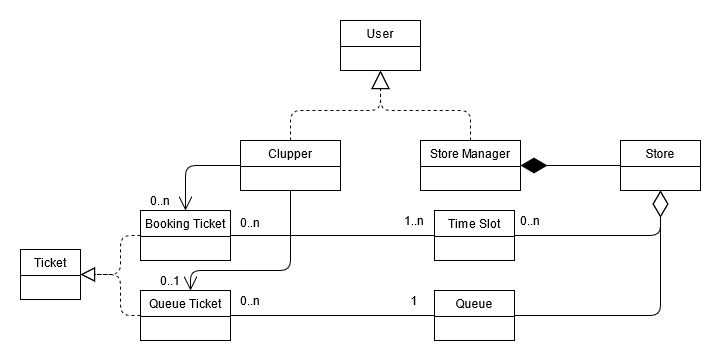
\includegraphics{assets/rasd/class_diagram/class_diagram_rasd.jpg}
\caption{Class diagram}
\end{figure}

\hypertarget{a.3.-state-diagrams}{%
\paragraph{A.3. State diagrams}\label{a.3.-state-diagrams}}

\hypertarget{a.3.1.-ticket-state}{%
\subparagraph{\texorpdfstring{A.3.1. Ticket state
}{A.3.1. Ticket state }}\label{a.3.1.-ticket-state}}

\begin{figure}
\centering
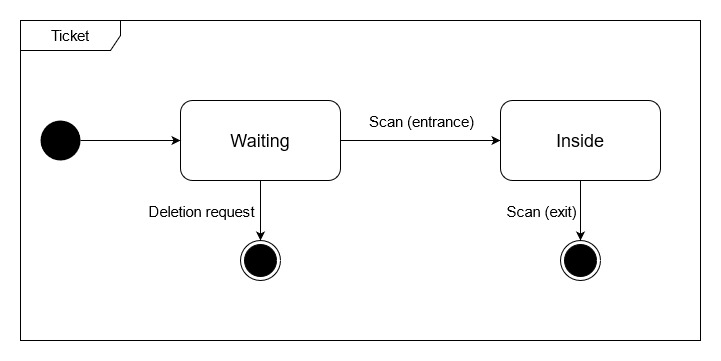
\includegraphics{assets/rasd/state_diagrams/ticket_state.jpg}
\caption{Ticket state}
\end{figure}

\hypertarget{a.3.2.-store-state}{%
\subparagraph{\texorpdfstring{A.3.2. Store state
}{A.3.2. Store state }}\label{a.3.2.-store-state}}

\begin{figure}
\centering
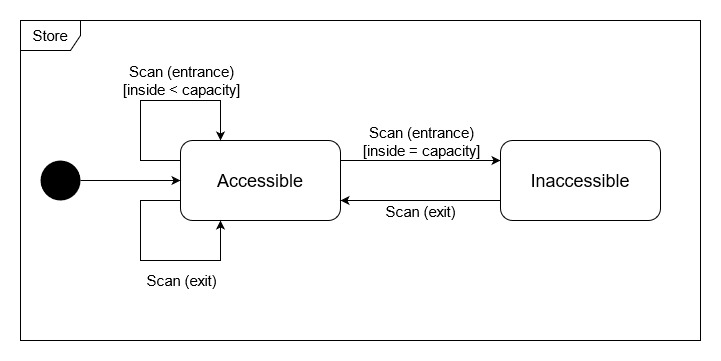
\includegraphics{assets/rasd/state_diagrams/store_state.jpg}
\caption{Store state}
\end{figure}

\hypertarget{a.3.3.-time-slot-state}{%
\subparagraph{\texorpdfstring{A.3.3. Time slot state
}{A.3.3. Time slot state }}\label{a.3.3.-time-slot-state}}

\begin{figure}
\centering
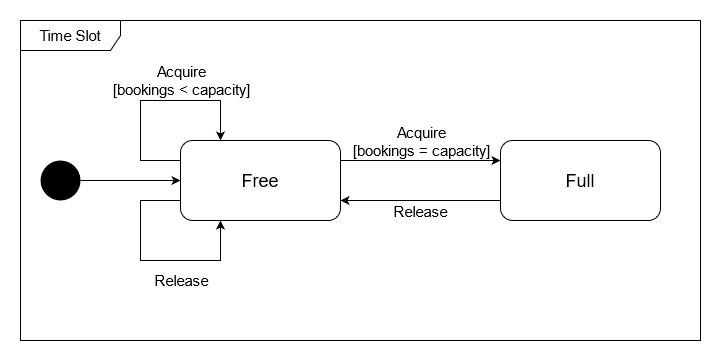
\includegraphics{assets/rasd/state_diagrams/time_slot_state.jpg}
\caption{Time slot state}
\end{figure}

\hypertarget{b.-product-functions}{%
\subsubsection{B. Product functions}\label{b.-product-functions}}

\hypertarget{b.1.-join-the-queue-digital---basic-service}{%
\paragraph{B.1. Join the queue (digital) - Basic
service}\label{b.1.-join-the-queue-digital---basic-service}}

This function allows a clupper to line up for the desired store without
having to immediately reach the store. After selecting a supermarket
from the map (searching around his GPS location or any address) the
clupper will be able to see its details (name, address, number of
customers already in line) and to join the queue. The system will
provide the clupper with a digital ticket, which he will be able to see
directly from the application. Finally, the clupper is able to leave the
queue at any time before entering the store, this results in the
deletion of his ticket.

\hypertarget{b.2.-book-a-visit---basic-service}{%
\paragraph{B.2. Book a visit - Basic
service}\label{b.2.-book-a-visit---basic-service}}

This function allows a clupper to book a visit to the desired store,
thus avoiding the queuing process. After selecting a supermarket from
the map (searching around his GPS location or any address) the clupper
will be able to see its details (name, address, number of customers
already in line) and to add a reservation. The system will request the
clupper to select one or more consecutive time slots and will provide
him with a digital ticket, which he will be able to see directly from
the application. Finally, the clupper is able to cancel his reservation
at any time before entering the store, this results in the deletion of
his ticket and the release of the acquired time slots.

\hypertarget{b.3.-join-the-queue-physical---managerial-service}{%
\paragraph{B.3. Join the queue (physical) - Managerial
service}\label{b.3.-join-the-queue-physical---managerial-service}}

This function is a fallback of the first one, indeed, it allows the
store manager to insert into the queue any guest requesting it. The
system will provide the store manager with a digital ticket, which he
will have to convert into physical (e.g.~by printing it) and hand out to
the guest.

\hypertarget{b.4.-store-overview---managerial-service}{%
\paragraph{B.4. Store overview - Managerial
service}\label{b.4.-store-overview---managerial-service}}

This function allows a store manager to have a live overview of the
store. The system will provide the store manager with the number of
customers inside the store (compared to the capacity), those in the
store queue and those with a reservation for the current time slot (that
have not entered the store yet). This data should allow him to regulate
the flow of customers.

\hypertarget{b.5.-ticket-scan---managerial-service}{%
\paragraph{B.5. Ticket scan - Managerial
service}\label{b.5.-ticket-scan---managerial-service}}

This function allows a store manager to scan (and validate) a customer's
ticket (both at the entrance and the exit of the store). This has the
double purpose of updating the data contained into the store overview,
and make sure that the flow of customers corresponds to that expected by
the system (no one should be able to enter before his turn).

\hypertarget{c.-user-characteristics}{%
\subsubsection{C. User characteristics}\label{c.-user-characteristics}}

\hypertarget{c.1.-clupper}{%
\paragraph{C.1. Clupper}\label{c.1.-clupper}}

Anyone who wants to become a clupper can do so by registering and
entering his personal information.\\
The main goal of a clupper is to avoid having to wait for his turn near
a store, thus reducing the risk of COVID infection.\\
To do so, the system offers a set of functions (called ``basic
services'') with which he is able to join a queue from wherever he wants
or to book a visit to enter the supermarket at a specific time.

\hypertarget{c.2.-store-manager}{%
\paragraph{C.2. Store manager}\label{c.2.-store-manager}}

Due to the higher privileges offered to him by the system, to become a
store manager a person shall enter, during the registration process,
specific information about his work place (thus adding the store to the
system).\\
The goal of a store manager is to avoid crowds inside the building by
limiting the flow of customers (to comply with current regulations).\\
To do so the system offers a set of functions (called ``managerial
services'') with which he is able to have an overview of the customers
dealing with the store and to approve their entrances.

\hypertarget{c.3.-other-stakeholders}{%
\paragraph{C.3. Other stakeholders}\label{c.3.-other-stakeholders}}

As explained in the previous sections, the system shall be able to
provide fallback options for customers that need to enter a store but do
not have access to the application. We define as \emph{guest} any person
who: - Is not registered to the system (regardless of whether they have
access to the required technology or not); - Is registered to the system
but is currently unable to use the application (e.g.~no device with him,
dead battery, no internet connection, \ldots);

The goal of a guest is the same as that of a clupper (the risk of
infection is technically lower due to the fact that the majority of
customers should be cluppers).\\
By definition, a guest cannot directly take advantage of the services
offered by the system, for this reason he is only able to join a queue
by addressing the store manager.

\hypertarget{d.-assumptions-dependencies-and-constraints}{%
\subsubsection{D. Assumptions, dependencies and
constraints}\label{d.-assumptions-dependencies-and-constraints}}

In order to better clarify the presentation and avoid any ambiguities we
decided to introduce the following assumptions.

\hypertarget{d.1.-text-assumptions}{%
\paragraph{D.1. Text assumptions}\label{d.1.-text-assumptions}}

\begin{itemize}
\tightlist
\item
  Credentials that a person has to provide to become a clupper are:
  name, surname, email and password.
\item
  Credentials that a person has to provide to become a store manager
  are: name, surname, email and password. He must also provide
  information about the store: name, address, VAT number, maximum
  capacity and opening time.
\item
  Credentials that a user has to provide to login are: email and
  password.
\item
  A User with a reservation can enter the store at any time during the
  booked time slots.
\end{itemize}

\hypertarget{d.2.-domain-assumptions}{%
\paragraph{D.2. Domain assumptions}\label{d.2.-domain-assumptions}}

\begin{longtable}[]{@{}
  >{\raggedright\arraybackslash}p{(\columnwidth - 2\tabcolsep) * \real{0.10}}
  >{\raggedright\arraybackslash}p{(\columnwidth - 2\tabcolsep) * \real{0.90}}@{}}
\toprule
DX & Description of the domain assumption \\ \addlinespace
\midrule
\endhead
D1 & The information provided by a user during the registration process
is valid \\ \addlinespace
D2 & The positions retrieved by GPS are always correct \\ \addlinespace
D3 & The store manager will always add to the store queue any guest
requesting it \\ \addlinespace
D4 & The store manager will always grant the precedence of a customer
with a reservation over those in the queue \\ \addlinespace
D5 & The store manager will always keep enough space inside the store to
accomodate the users with a reservation \\ \addlinespace
D6 & At any time during the visit to a store, the customer shall be able
to show the ticket with which he entered to the store
manager \\ \addlinespace
D7 & A clupper with a reservation should leave the store before the end
of the acquired time slots \\ \addlinespace
D8 & A customer is not able to enter a store before providing a valid
ticket to the store manager \\ \addlinespace
D9 & A customer is not able to leave a store before providing a valid
ticket to the store manager \\ \addlinespace
\bottomrule
\end{longtable}

\hypertarget{secific-requirements}{%
\subsection{3. Secific requirements}\label{secific-requirements}}

\hypertarget{a.-external-interface-requirements}{%
\subsubsection{A. External interface
requirements}\label{a.-external-interface-requirements}}

\hypertarget{a.1.-user-interfaces}{%
\paragraph{A.1. User interfaces}\label{a.1.-user-interfaces}}

The following mockups represent an idea of what the application shall
look like in the first release.

TODO

\hypertarget{a.2.-hardware-interfaces}{%
\paragraph{A.2. Hardware interfaces}\label{a.2.-hardware-interfaces}}

The system requires each clupper to have at least one mobile device
(such as a smartphone or tablet) that will be used to exibit the ticket
to the store manager.\\
The clupper can perform the operations to obtain a ticket also from a PC
of any kind that will however not be sufficient to have access to the
store.

The store manager needs a mobile device or a PC equipped with a camera
to scan the tickets and a printer of any kind to hand out tickets to the
guests.

\hypertarget{a.3.-software-interfaces}{%
\paragraph{A.3. Software interfaces}\label{a.3.-software-interfaces}}

The CLup applicative is a web application, for this reason a relatively
modern web browser is sufficient in order to render the application.

\hypertarget{a.4.-communication-interfaces}{%
\paragraph{A.4. Communication
interfaces}\label{a.4.-communication-interfaces}}

To perform any operation in the application, an Internet connection
(WiFi or mobile) is required.\\
When a clupper has queued-up or has booked for a visit, can interrupt
the connection without losing the place in the queue or the booking (he
will not have access to the live information such as place in the queue
or expected waiting time).

A store manager always needs a stable internet connection in order to
have access to the managerial services.

\hypertarget{b.-functional-requirements}{%
\subsubsection{B. Functional
requirements}\label{b.-functional-requirements}}

\begin{longtable}[]{@{}
  >{\raggedright\arraybackslash}p{(\columnwidth - 2\tabcolsep) * \real{0.09}}
  >{\raggedright\arraybackslash}p{(\columnwidth - 2\tabcolsep) * \real{0.91}}@{}}
\toprule
RX & Description of the functional requirement \\ \addlinespace
\midrule
\endhead
R1 & A person is able to register to the system as a user. During the
process, the system will ask him to provide the information required for
the specific type of user \\ \addlinespace
R2 & The system is able to verify that the email provided by a person
during the registration process is unique \\ \addlinespace
R3 & The system is able to verify that the VAT number provided by a
store manager during the registration process is unique \\ \addlinespace
R4 & The system is able to create a new store after the registration of
store manager \\ \addlinespace
R5 & A user is able to log into the system by entering his personal
credentials \\ \addlinespace
R6 & The system is able to generate a new ticket after receiving a
request \\ \addlinespace
R7 & A clupper is able to join at most one queue at any time (for any
store) \\ \addlinespace
R8 & The system is able to insert a ticket into a store
queue \\ \addlinespace
R9 & The system is able to remove a ticket from a store
queue \\ \addlinespace
R10 & A clupper is able to select as many consecutive free time slots as
he wants while booking a visit to a store \\ \addlinespace
R11 & A clupper cannot have multiple reservations in the same time
slots \\ \addlinespace
R12 & The system is able to retrieve the list of free time slots for
each store \\ \addlinespace
R13 & The system is able to acquire the selected free time slots when
creating a new reservation to a store \\ \addlinespace
R14 & The system is able to release the time slots acquired by a
reservation when a clupper cancels it \\ \addlinespace
R15 & The system is able to notify a clupper the time in which he should
approach the store \\ \addlinespace
R16 & A clupper is able to retrieve a previously obtained
ticket \\ \addlinespace
R17 & A store manager is able to change the maximum store capacity at
any time \\ \addlinespace
R18 & The system is able to infer the number of time slots to be
proposed to a clupper when booking a visit to the store \\ \addlinespace
R19 & A store manager is able to scan a customer's ticket at the
entrance of the store before letting him in only if the number of
customers currently inside does not exceed its maximum
capacity \\ \addlinespace
R20 & A store manager is always able to scan a customer's ticket at the
exit of the store before letting him out \\ \addlinespace
R21 & The system is able to perform a validity check on a ticket scanned
by a store manager and to inform him about the result \\ \addlinespace
R22 & The system is able to remove a customer's ticket from the store
queue when it is scanned at the entrance \\ \addlinespace
R23 & The system is able to invalidate a customer's ticket when it is
scanned at the exit \\ \addlinespace
R24 & The system is able to retrieve the customer's GPS
location \\ \addlinespace
R25 & The system is able to retrieve the GPS location from a specific
address \\ \addlinespace
R26 & The system is able to estimate the distance between two GPS
locations \\ \addlinespace
R27 & The system is able to get a list of stores around a GPS
location \\ \addlinespace
R28 & The system is able to retrieve the name and GPS location of a
store \\ \addlinespace
R29 & The system is able to retrieve the position of a clupper in a
store queue \\ \addlinespace
R30 & The system is able to estimate the waiting time for a clupper in a
store queue \\ \addlinespace
R31 & The system is able to retrieve the number of customers currently
in a store queue \\ \addlinespace
R32 & The system is able to retrieve the number of customers currently
inside a store \\ \addlinespace
R33 & The system is able to retrieve the number of reservations for a
store during the current time slot \\ \addlinespace
\bottomrule
\end{longtable}

\hypertarget{b.1.-use-cases}{%
\paragraph{B.1. Use cases}\label{b.1.-use-cases}}

\begin{longtable}[]{@{}
  >{\raggedright\arraybackslash}p{(\columnwidth - 2\tabcolsep) * \real{0.20}}
  >{\raggedright\arraybackslash}p{(\columnwidth - 2\tabcolsep) * \real{0.80}}@{}}
\toprule
VisitorRegisters & \\ \addlinespace
\midrule
\endhead
Actors & Visitor \\ \addlinespace
Goals & G1, G4, G7 \\ \addlinespace
Input conditions & The visitor is already on the home
page. \\ \addlinespace
Events flow & 1. The visitor clicks on the ``Sign Up'' button to start
the registration process.2. The visitor inserts his information in the
mandatory fields.3. The visitor clicks the ``Register'' button.4. The
system stores the inserted data.5. The system redirects the visitor to
the login page. \\ \addlinespace
Output conditions & The visitor successfully ends the registration
process and becomes a CLup user. From now on he can login to the
application providing his credentials and use CLup. \\ \addlinespace
Exceptions & 1. The provided email is already registered.2. The visitor
inserts not valid informations in one or more mandatory fields.All
exceptions are handled notifying the issue to the visitor and taking
back the event flow to the point 2. \\ \addlinespace
\bottomrule
\end{longtable}

\begin{longtable}[]{@{}
  >{\raggedright\arraybackslash}p{(\columnwidth - 2\tabcolsep) * \real{0.20}}
  >{\raggedright\arraybackslash}p{(\columnwidth - 2\tabcolsep) * \real{0.80}}@{}}
\toprule
UserLogsIn & \\ \addlinespace
\midrule
\endhead
Actors & User \\ \addlinespace
Goals & G1, G2, G3, G4, G5, G6, G7, G8, G9 \\ \addlinespace
Input conditions & The user is already on the home
page. \\ \addlinespace
Events flow & 1. The user clicks on the ``Sign In'' button to start the
login process.2. The User inserts his email and password into the
corresponding fields.3. The user clicks the ``Login'' button.4. The
system redirects the user to the map page. \\ \addlinespace
Output conditions & The user successfully logs in. From now on he can
use the CLup services. \\ \addlinespace
Exceptions & 1. The inserted email is not valid.2. The inserted password
is not valid.All exceptions are handled notifying the issue to the user
and taking back the event flow to the point 2. \\ \addlinespace
Alternatives & If the user is a store manager:4. The system redirects
the user to the overview page. \\ \addlinespace
\bottomrule
\end{longtable}

\begin{longtable}[]{@{}
  >{\raggedright\arraybackslash}p{(\columnwidth - 2\tabcolsep) * \real{0.20}}
  >{\raggedright\arraybackslash}p{(\columnwidth - 2\tabcolsep) * \real{0.80}}@{}}
\toprule
ClupperSelectsStore & \\ \addlinespace
\midrule
\endhead
Actors & Clupper \\ \addlinespace
Goals & G1, G4 \\ \addlinespace
Input conditions & The clupper is already logged in and on the map
page. \\ \addlinespace
Events flow & 1. The clupper inserts an address or clicks on the
``Current Position'' button2. The system retrieves the GPS location and
loads the stores on the map 3. The clupper looks at the map and selects
one of the available stores.4. The system redirects the clupper to the
store page. \\ \addlinespace
Output conditions & The clupper successfully selects the store. Now he
can see its details, queue up or book a visit for it. \\ \addlinespace
Exceptions & 1. The system does not contain any store.All exceptions are
handled notifying the issue to the clupper and redirecting him to the
map page. \\ \addlinespace
\bottomrule
\end{longtable}

\begin{longtable}[]{@{}
  >{\raggedright\arraybackslash}p{(\columnwidth - 2\tabcolsep) * \real{0.20}}
  >{\raggedright\arraybackslash}p{(\columnwidth - 2\tabcolsep) * \real{0.80}}@{}}
\toprule
ClupperJoinsQueue & \\ \addlinespace
\midrule
\endhead
Actors & Clupper \\ \addlinespace
Goals & G1 \\ \addlinespace
Input conditions & The clupper is already logged in, has chosen the
desired store and is on its page. \\ \addlinespace
Events flow & 1. The clupper clicks on the ``Line Up'' button on the
store page.2. The system generates a ticket and adds it to the store
queue.3. The system redirects the clupper to the queue
page. \\ \addlinespace
Output conditions & The clupper is successfully in the store
queue. \\ \addlinespace
Exceptions & 1. The clupper is already in a queue.All exceptions are
handled notifying the issue to the clupper and redirecting him to the
map page. \\ \addlinespace
\bottomrule
\end{longtable}

\begin{longtable}[]{@{}
  >{\raggedright\arraybackslash}p{(\columnwidth - 2\tabcolsep) * \real{0.20}}
  >{\raggedright\arraybackslash}p{(\columnwidth - 2\tabcolsep) * \real{0.80}}@{}}
\toprule
ClupperLeavesQueue & \\ \addlinespace
\midrule
\endhead
Actors & Clupper \\ \addlinespace
Goals & G3 \\ \addlinespace
Input conditions & The clupper is already logged into the system and in
the queue page. \\ \addlinespace
Events flow & 1. The clupper clicks on the ``Leave the Queue'' button.2.
The system removes the clupper's ticket from the store queue and deletes
it.3. The system redirects the clupper to the map page. \\ \addlinespace
Output conditions & The clupper is no longer in the store
queue. \\ \addlinespace
Exceptions & 1. The clupper is not currently in a queue.All exceptions
are handled notifying the issue to the clupper and redirecting him to
the queue page. \\ \addlinespace
\bottomrule
\end{longtable}

\begin{longtable}[]{@{}
  >{\raggedright\arraybackslash}p{(\columnwidth - 2\tabcolsep) * \real{0.20}}
  >{\raggedright\arraybackslash}p{(\columnwidth - 2\tabcolsep) * \real{0.80}}@{}}
\toprule
ClupperWatchesTicketDetails & \\ \addlinespace
\midrule
\endhead
Actors & Clupper \\ \addlinespace
Goals & G6, G8, G9 \\ \addlinespace
Input conditions & The clupper is already logged in. \\ \addlinespace
Events flow & 1. The clupper clicks goes to the queue page or the
reservations page depending on the type of ticket that he wants to
watch.2. If the clupper is in the reserviations page, he selects a
ticket from the list of bookings.3. The system fetches the details of
the selected ticket.4. The system redirects the clupper to the ticket
page. \\ \addlinespace
Output conditions & The clupper can see ticket details. \\ \addlinespace
Exceptions & 1. The clupper is not currently in a queue. 2 The clupper
doesn't have an active booking.All exceptions are handled notifying the
issue to the clupper and redirecting him to the queue
page. \\ \addlinespace
\bottomrule
\end{longtable}

\begin{longtable}[]{@{}
  >{\raggedright\arraybackslash}p{(\columnwidth - 2\tabcolsep) * \real{0.20}}
  >{\raggedright\arraybackslash}p{(\columnwidth - 2\tabcolsep) * \real{0.80}}@{}}
\toprule
ClupperBooksVisit & \\ \addlinespace
\midrule
\endhead
Actors & Clupper \\ \addlinespace
Goals & G4 \\ \addlinespace
Input conditions & The clupper is already logged in, has chosen the
desired store and is on its page. \\ \addlinespace
Events flow & 1. The clupper clicks on the ``Book a Visit'' button on
the store page.2. The clupper selects one or more avaiable time slots.3.
The system generates a ticket and acquires the selected time slots.4.
The system redirects the clupper to the reservations
page. \\ \addlinespace
Output conditions & The clupper has a reservation for the
store. \\ \addlinespace
Exceptions & 1. The clupper has already a reservation during one of the
selected time slots.2. One or more of the selected time slots is not
free.All exceptions are handled notifying the issue to the clupper and
taking back the event flow to the point 2. \\ \addlinespace
\bottomrule
\end{longtable}

\begin{longtable}[]{@{}
  >{\raggedright\arraybackslash}p{(\columnwidth - 2\tabcolsep) * \real{0.21}}
  >{\raggedright\arraybackslash}p{(\columnwidth - 2\tabcolsep) * \real{0.79}}@{}}
\toprule
ClupperCancelsVisit & \\ \addlinespace
\midrule
\endhead
Actors & Clupper \\ \addlinespace
Goals & G5 \\ \addlinespace
Input conditions & The clupper is already logged into the system and in
the reservations page. \\ \addlinespace
Events flow & 1. The clupper looks at the list of active reservations.2.
The clupper selects the booking he wants to cancel.3. The clupper clicks
on the ``Cancel Booking'' button.3. The system removes the clupper's
ticket from the store reservations and deletes it.4. The system
redirects the clupper to the reservations page. \\ \addlinespace
Output conditions & The clupper has no longer a reservation for that
store. \\ \addlinespace
Exceptions & 1. The clupper does not have a reservation for that
store.All exceptions are handled notifying the issue to the clupper and
redirecting him to the reservations page. \\ \addlinespace
\bottomrule
\end{longtable}

\begin{longtable}[]{@{}
  >{\raggedright\arraybackslash}p{(\columnwidth - 2\tabcolsep) * \real{0.20}}
  >{\raggedright\arraybackslash}p{(\columnwidth - 2\tabcolsep) * \real{0.80}}@{}}
\toprule
StoreManagerPrintsTicket & \\ \addlinespace
\midrule
\endhead
Actors & Store manager, Guest \\ \addlinespace
Goals & G2 \\ \addlinespace
Input conditions & The store manager is already logged into the system
and in the overview page. \\ \addlinespace
Events flow & 1. The guest approaches the store manager asking for a
ticket.2. The store manager clicks on the ``Issue Ticket'' button.3. The
system generates a ticket and adds it to the store queue4. The system
redirects the store manager to the ticket page.4. The store manager
clicks on the ``Print Ticket'' button \\ \addlinespace
Output conditions & The store manager is able to print the newly issued
ticket and hand it out to the guest. \\ \addlinespace
Exceptions & \emph{None} \\ \addlinespace
Special Requirements & The Store Manager's device must be connected to a
printer. \\ \addlinespace
\bottomrule
\end{longtable}

\begin{longtable}[]{@{}
  >{\raggedright\arraybackslash}p{(\columnwidth - 2\tabcolsep) * \real{0.20}}
  >{\raggedright\arraybackslash}p{(\columnwidth - 2\tabcolsep) * \real{0.80}}@{}}
\toprule
StoreManagerScansTicket & \\ \addlinespace
\midrule
\endhead
Actors & Store manager, Customer \\ \addlinespace
Goals & G8, G9 \\ \addlinespace
Input conditions & The store manager is already logged into the system
and in the overview page. \\ \addlinespace
Events flow & 1. The store manager clicks on the ``Scan Ticket''
button.2. The store manager uses the device camera to scan the
customer's ticket.3. The system validates and removes the ticket from
the store queue or the list of reservations.4. The system updates the
store overview data.5. The system redirects the store manager to the
overview page. \\ \addlinespace
Output conditions & The store manager can let the customer in/out. The
store overview has been updated. \\ \addlinespace
Exceptions & 1. The store has reached its maximum capacity and cannot
allow any other Customer inside.2. The ticket is invalid.All exceptions
are handled notifying the issue to the Store Manager and redirecting him
to the overview page. \\ \addlinespace
Special Requirements & The Store Manager's device must be connected to a
camera. \\ \addlinespace
\bottomrule
\end{longtable}

\begin{longtable}[]{@{}
  >{\raggedright\arraybackslash}p{(\columnwidth - 2\tabcolsep) * \real{0.20}}
  >{\raggedright\arraybackslash}p{(\columnwidth - 2\tabcolsep) * \real{0.80}}@{}}
\toprule
StoreManagerGetsOverview & \\ \addlinespace
\midrule
\endhead
Actors & Store manager \\ \addlinespace
Goals & G7 \\ \addlinespace
Input conditions & The store manager is already logged into the system
and in the overview page. \\ \addlinespace
Events flow & 1. The system loads up the details about the store and
displays it into the overview page. \\ \addlinespace
Output conditions & The store manager is able see the details about his
store. \\ \addlinespace
Exceptions & \emph{None} \\ \addlinespace
\bottomrule
\end{longtable}

\hypertarget{b.2.-use-case-diagrams}{%
\paragraph{B.2. Use case diagrams}\label{b.2.-use-case-diagrams}}

\hypertarget{b.2.1-visitor}{%
\subparagraph{\texorpdfstring{B.2.1 Visitor
}{B.2.1 Visitor }}\label{b.2.1-visitor}}

\begin{figure}
\centering
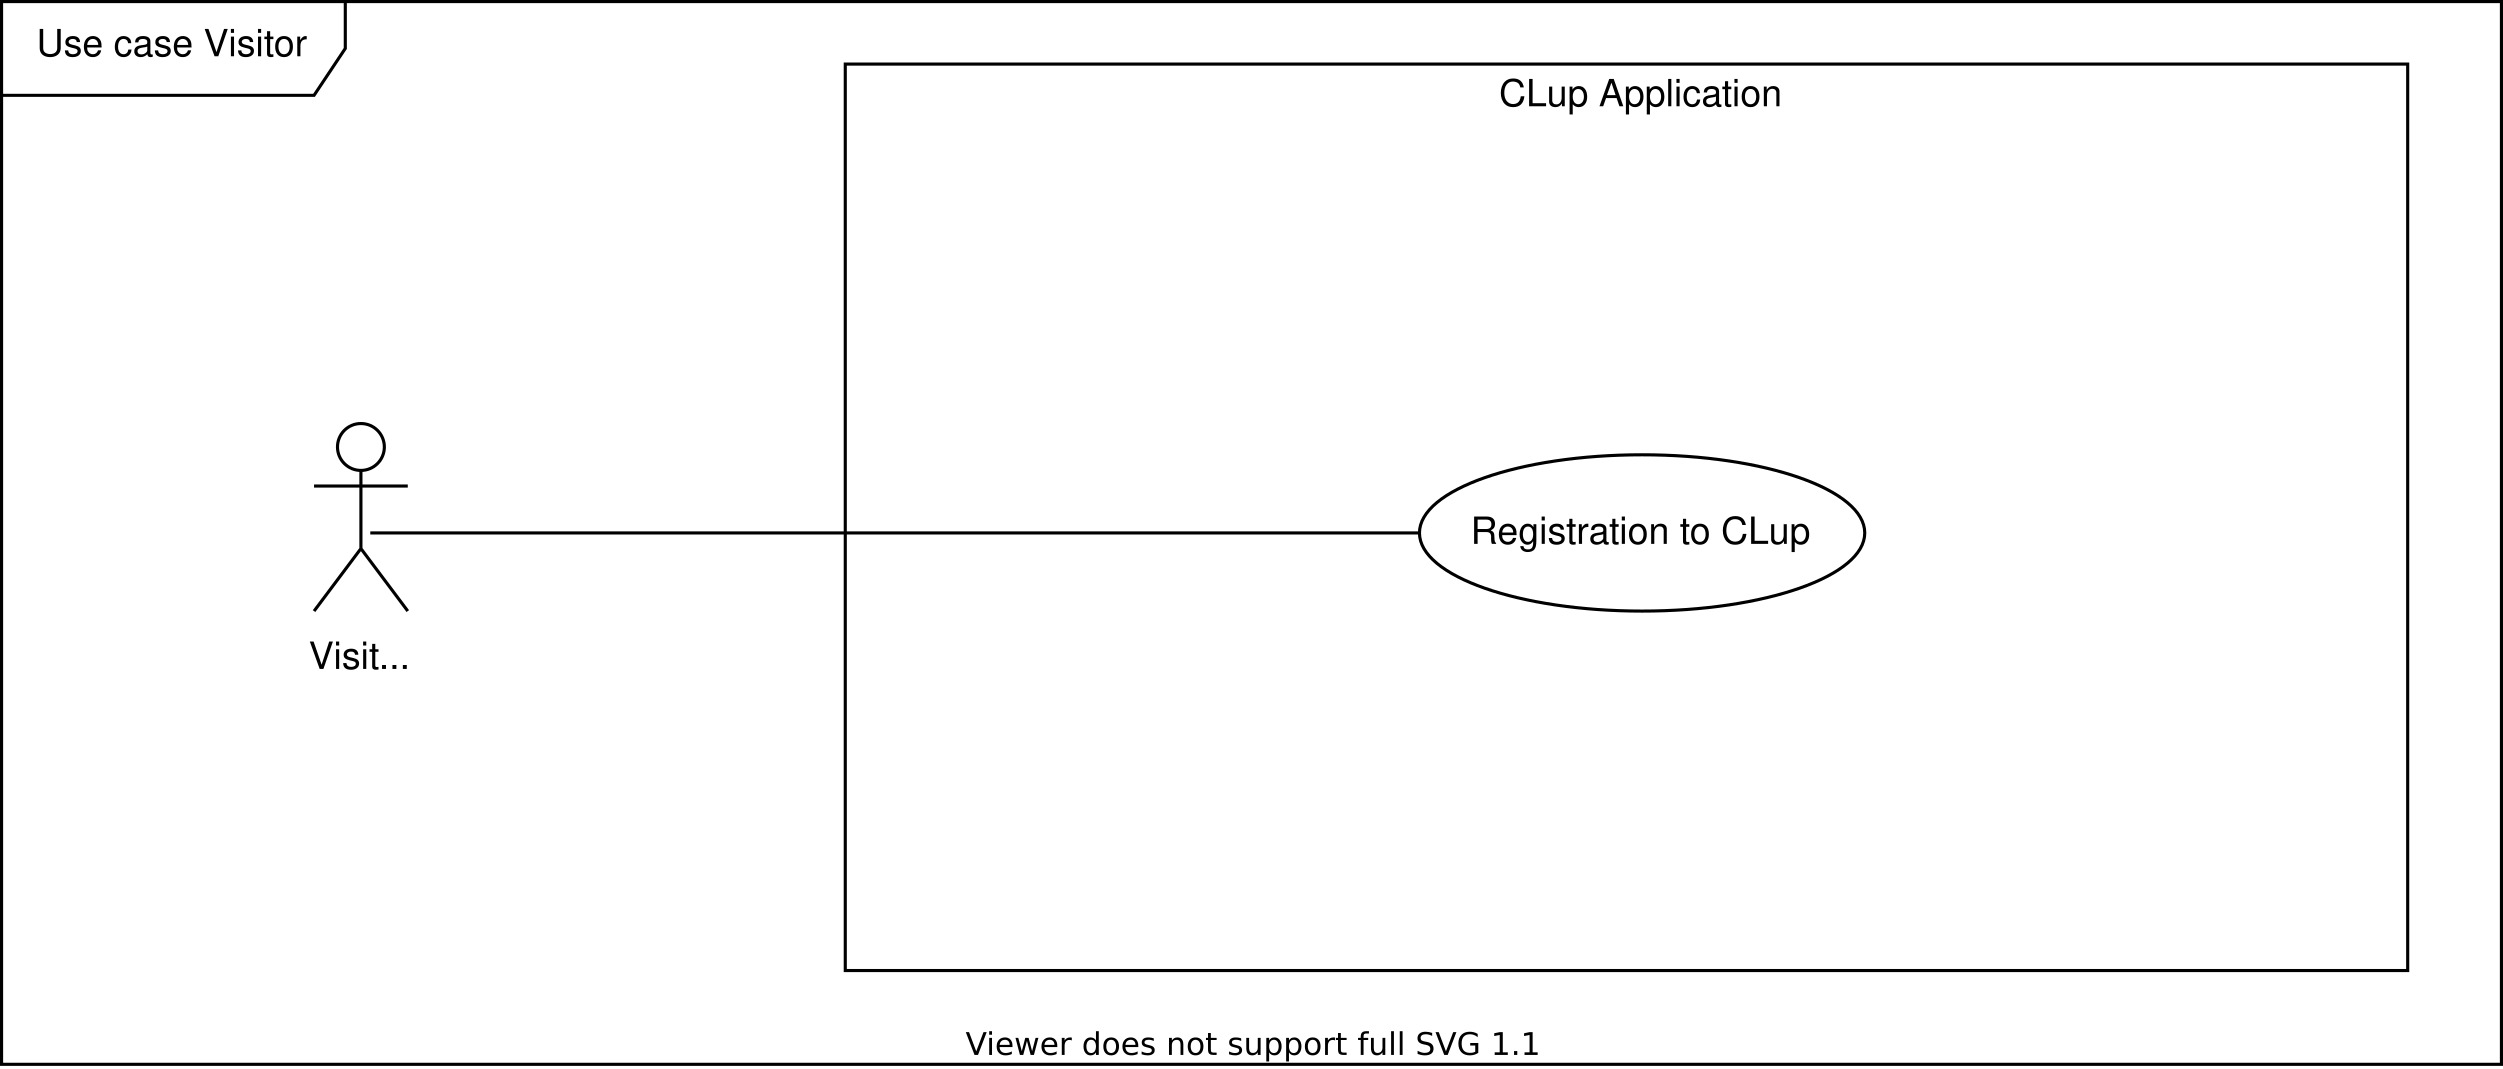
\includegraphics{assets/rasd/use_cases/use_case_visitor_registration.jpg}
\caption{Visitor}
\end{figure}

\hypertarget{b.2.2-user}{%
\subparagraph{\texorpdfstring{B.2.2 User
}{B.2.2 User }}\label{b.2.2-user}}

\begin{figure}
\centering
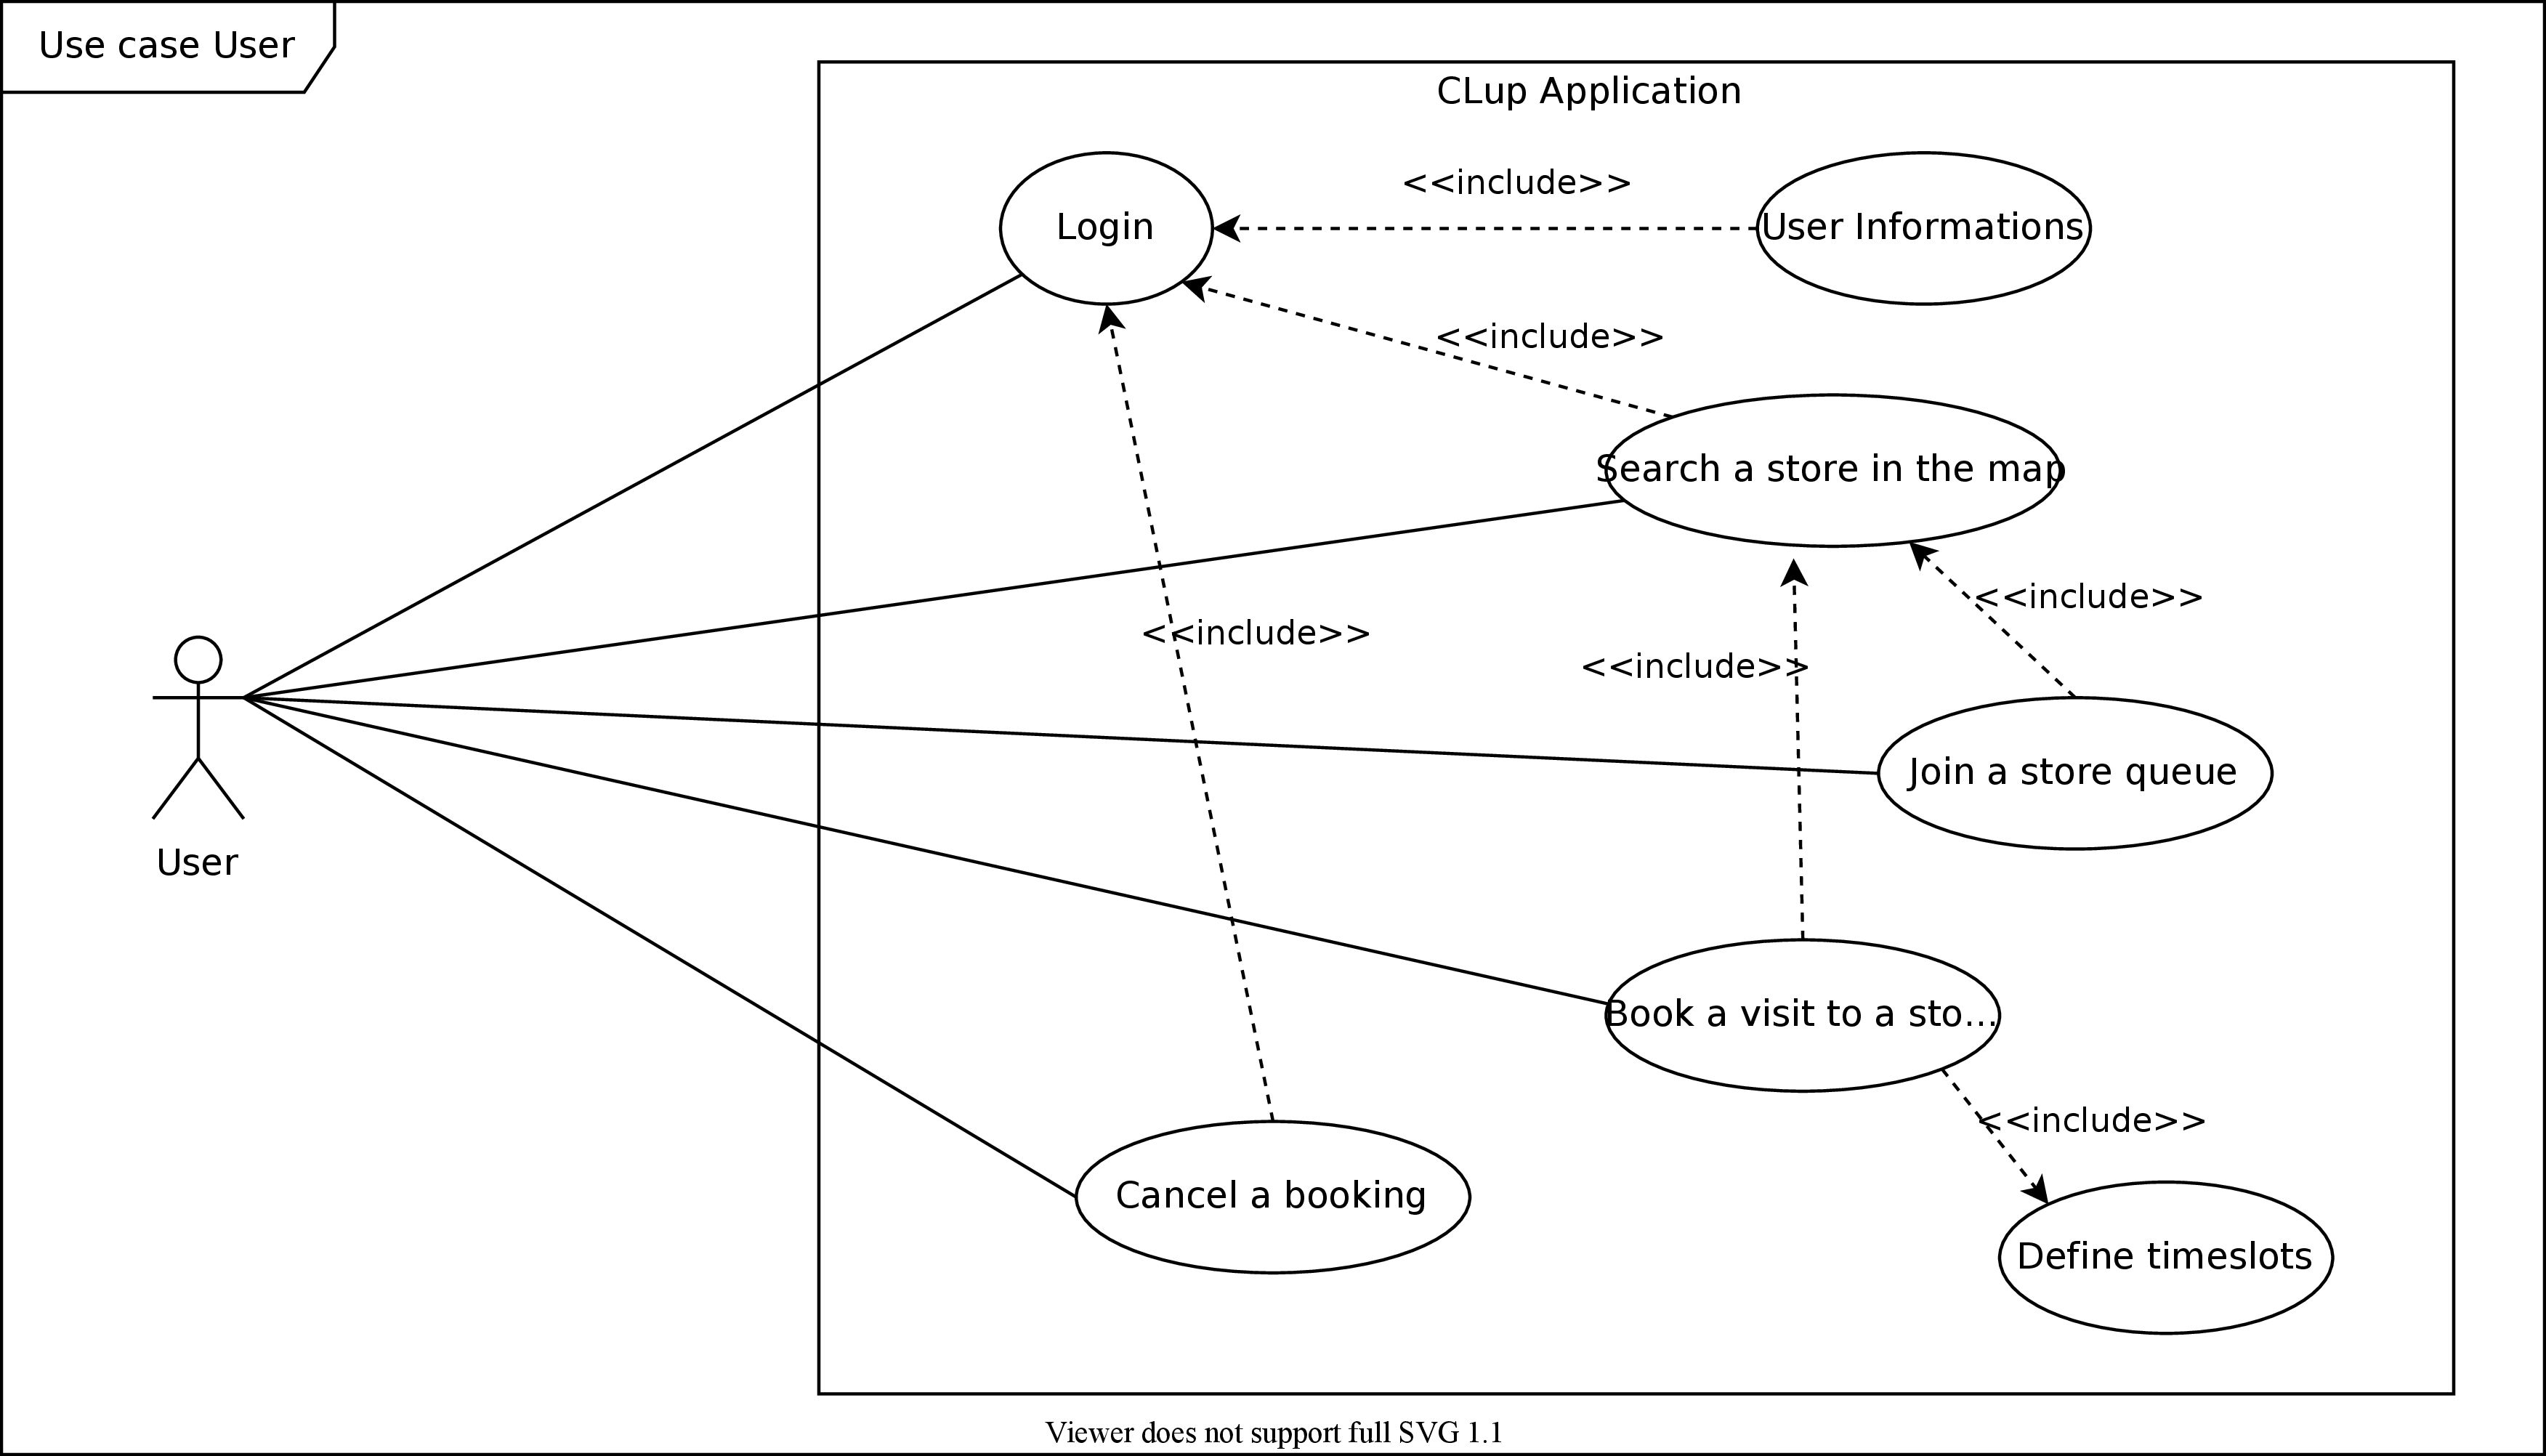
\includegraphics{assets/rasd/use_cases/use_case_user.jpg}
\caption{User}
\end{figure}

\hypertarget{b.2.2-store-manager}{%
\subparagraph{\texorpdfstring{B.2.2 Store Manager
}{B.2.2 Store Manager }}\label{b.2.2-store-manager}}

\begin{figure}
\centering
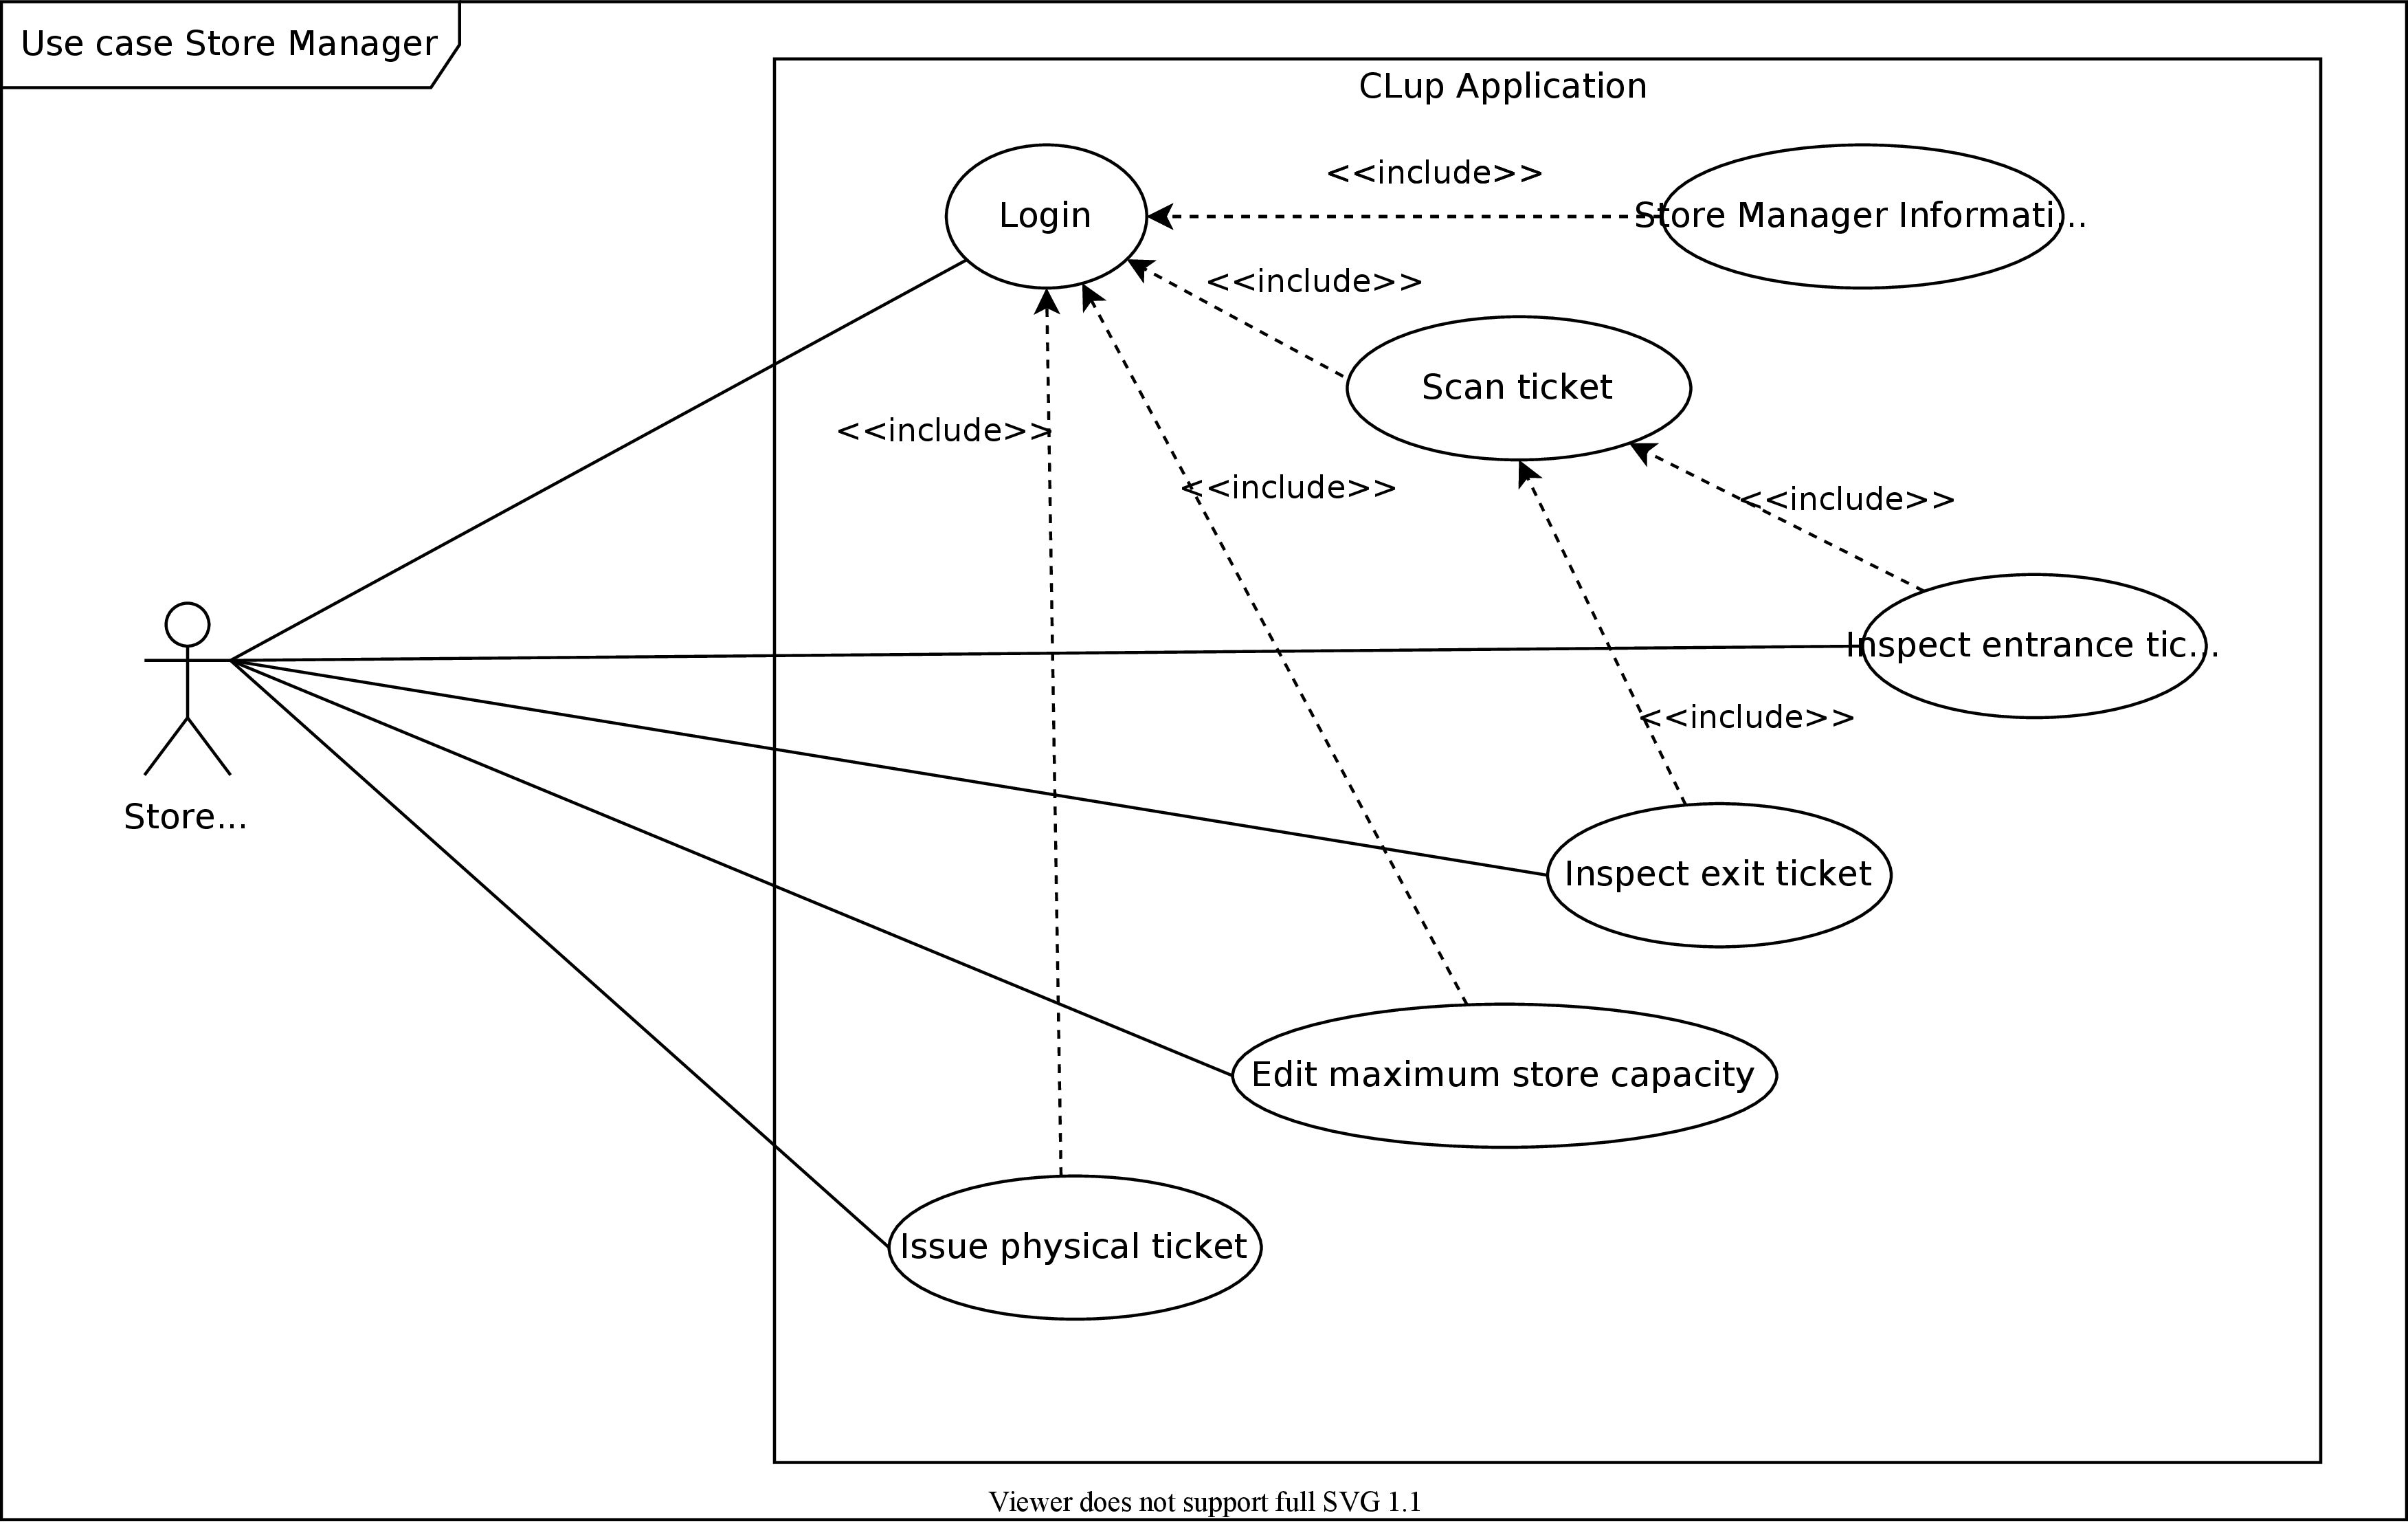
\includegraphics{assets/rasd/use_cases/use_case_store_manager.jpg}
\caption{Store Manager}
\end{figure}

\hypertarget{b.3.-sequence-diagrams}{%
\paragraph{B.3. Sequence diagrams}\label{b.3.-sequence-diagrams}}

\hypertarget{b.3.1-visitor-registration}{%
\subparagraph{\texorpdfstring{B.3.1 Visitor Registration
}{B.3.1 Visitor Registration }}\label{b.3.1-visitor-registration}}

\begin{figure}
\centering
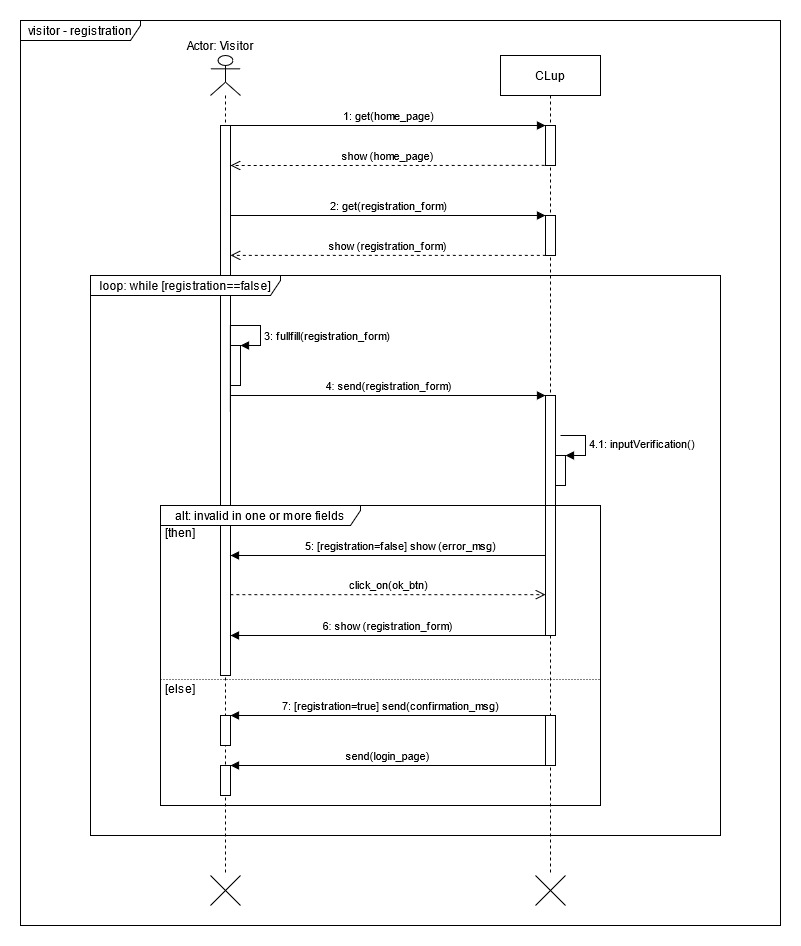
\includegraphics{assets/rasd/sequence_diagrams/sequence_diagram_visitor_registration.jpg}
\caption{Visitor Registration}
\end{figure}

\hypertarget{b.3.2-user-login}{%
\subparagraph{\texorpdfstring{B.3.2 User Login
}{B.3.2 User Login }}\label{b.3.2-user-login}}

\begin{figure}
\centering
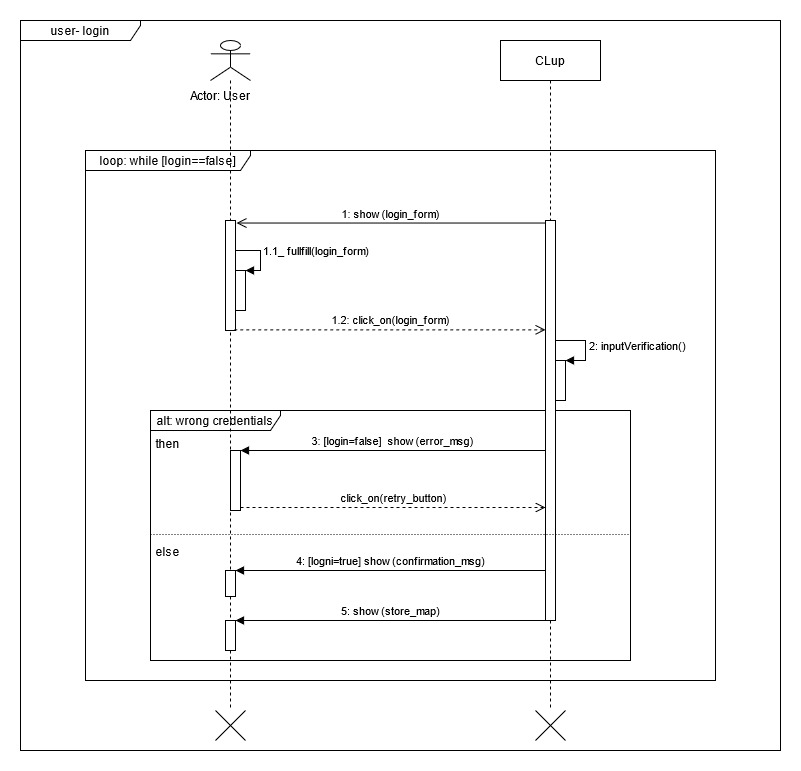
\includegraphics{assets/rasd/sequence_diagrams/sequence_diagram_user_login.jpg}
\caption{User Login}
\end{figure}

\hypertarget{b.3.3-user-queue-up}{%
\subparagraph{\texorpdfstring{B.3.3 User Queue Up
}{B.3.3 User Queue Up }}\label{b.3.3-user-queue-up}}

\begin{figure}
\centering
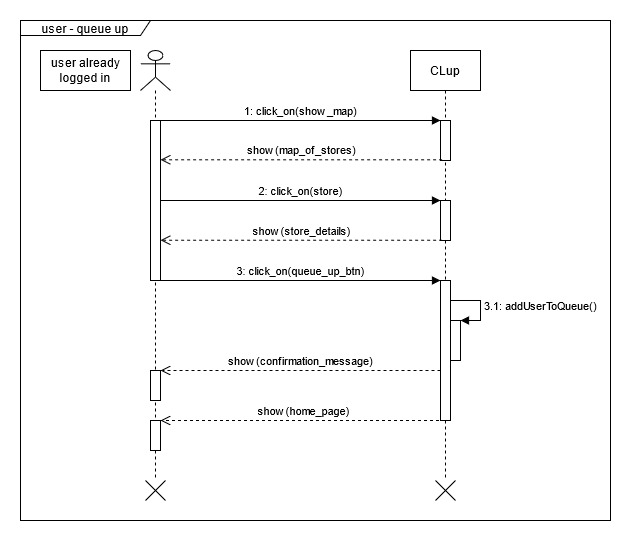
\includegraphics{assets/rasd/sequence_diagrams/sequence_diagram_user_queue_up.jpg}
\caption{User Queue Up}
\end{figure}

\hypertarget{b.3.4-user-leave-queue}{%
\subparagraph{\texorpdfstring{B.3.4 User Leave Queue
}{B.3.4 User Leave Queue }}\label{b.3.4-user-leave-queue}}

\begin{figure}
\centering
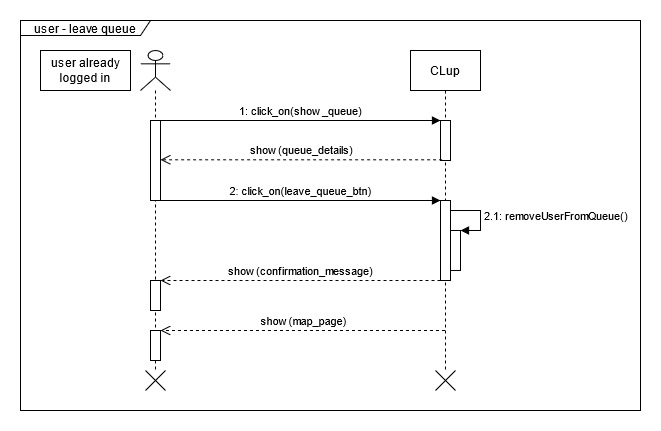
\includegraphics{assets/rasd/sequence_diagrams/sequence_diagram_user_leave_queue.jpg}
\caption{User Leave Queue}
\end{figure}

\hypertarget{b.3.5-user-booking-a-visit}{%
\subparagraph{\texorpdfstring{B.3.5 User Booking a Visit
}{B.3.5 User Booking a Visit }}\label{b.3.5-user-booking-a-visit}}

\begin{figure}
\centering
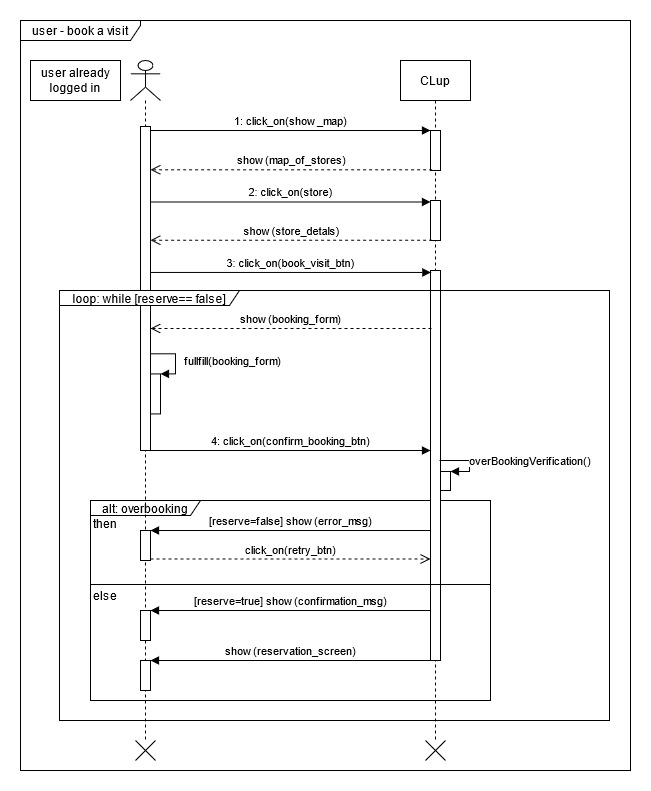
\includegraphics{assets/rasd/sequence_diagrams/sequence_diagram_user_booking.jpg}
\caption{Booking a Visit}
\end{figure}

\hypertarget{b.3.6-user-cancels-a-booking}{%
\subparagraph{\texorpdfstring{B.3.6 User Cancels a Booking
}{B.3.6 User Cancels a Booking }}\label{b.3.6-user-cancels-a-booking}}

\begin{figure}
\centering
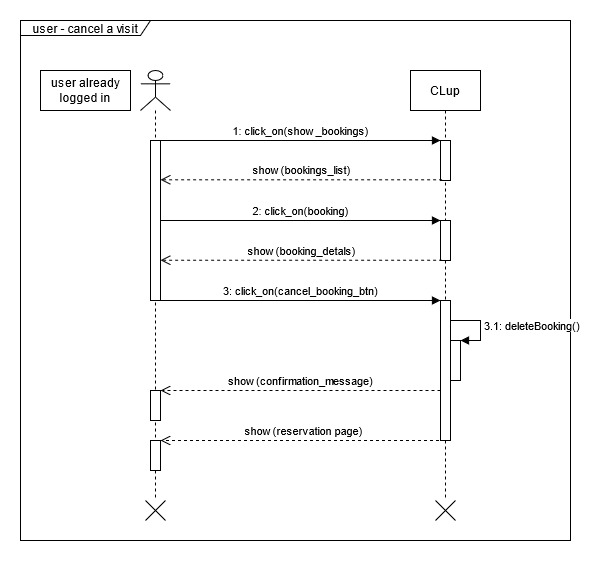
\includegraphics{assets/rasd/sequence_diagrams/sequence_diagram_user_cancel_booking.jpg}
\caption{User Cancels a Booking}
\end{figure}

\hypertarget{b.3.7-store-manager-issue-ticket}{%
\subparagraph{\texorpdfstring{B.3.7 Store Manager Issue Ticket
}{B.3.7 Store Manager Issue Ticket }}\label{b.3.7-store-manager-issue-ticket}}

\begin{figure}
\centering
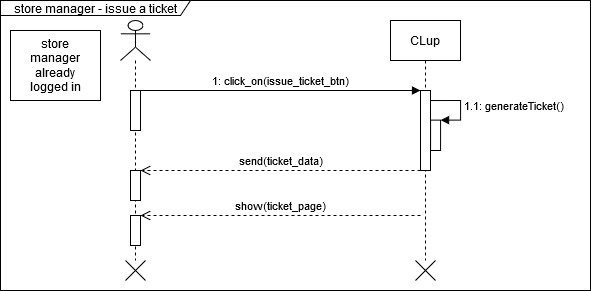
\includegraphics{assets/rasd/sequence_diagrams/sequence_diagram_store_manager_issue_ticket.jpg}
\caption{Store Manager Issue Ticket}
\end{figure}

\hypertarget{b.3.7-store-manager-scan-ticket}{%
\subparagraph{\texorpdfstring{B.3.7 Store Manager Scan Ticket
}{B.3.7 Store Manager Scan Ticket }}\label{b.3.7-store-manager-scan-ticket}}

\begin{figure}
\centering
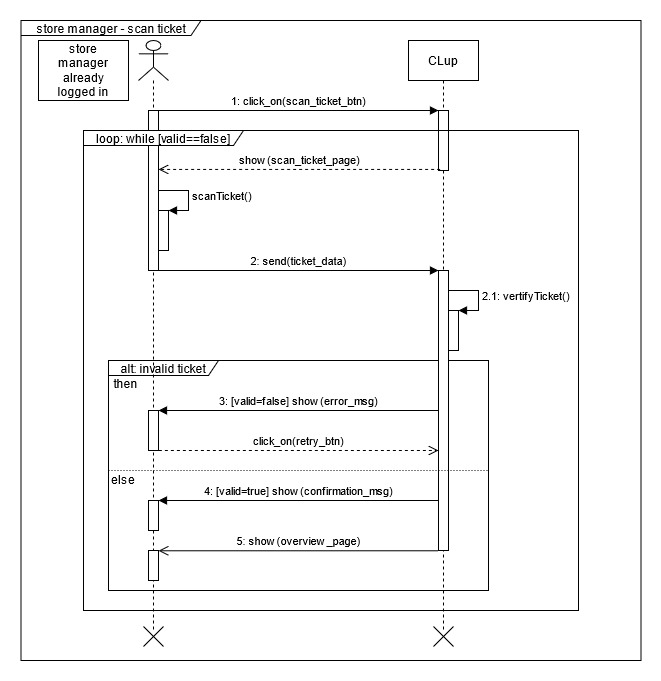
\includegraphics{assets/rasd/sequence_diagrams/sequence_diagram_store_manager_scan_ticket.jpg}
\caption{Store Manager Scan Ticket}
\end{figure}

\hypertarget{b.4.-mapping-on-requirements}{%
\paragraph{B.4. Mapping on
requirements}\label{b.4.-mapping-on-requirements}}

\begin{longtable}[]{@{}
  >{\raggedright\arraybackslash}p{(\columnwidth - 2\tabcolsep) * \real{0.03}}
  >{\raggedright\arraybackslash}p{(\columnwidth - 2\tabcolsep) * \real{0.97}}@{}}
\toprule
G1 & Allow a clupper to join a store queue without having to physically
approach the store \\ \addlinespace
\midrule
\endhead
D1 & The information provided by a user during the registration process
is valid \\ \addlinespace
D2 & The positions retrieved by GPS are always correct \\ \addlinespace
R1 & A person is able to register to the system as a user. During the
process, the system will ask him to provide the information required for
the specific type of user \\ \addlinespace
R2 & The system is able to verify that the email provided by a person
during the registration process is unique \\ \addlinespace
R5 & A user is able to log into the system by entering his personal
credentials \\ \addlinespace
R6 & The system is able to generate a new ticket after receiving a
request \\ \addlinespace
R7 & A clupper is able to join at most one queue at any time (for any
store) \\ \addlinespace
R8 & The system is able to insert a ticket into a store
queue \\ \addlinespace
R24 & The system is able to retrieve the customer's GPS
location \\ \addlinespace
R25 & The system is able to retrieve the GPS location from a specific
address \\ \addlinespace
R26 & The system is able to estimate the distance between two GPS
locations \\ \addlinespace
R27 & The system is able to get a list of stores around a GPS
location \\ \addlinespace
R28 & The system is able to retrieve the name and GPS location of a
store \\ \addlinespace
R31 & The system is able to retrieve the number of customers currently
in a store queue \\ \addlinespace
\bottomrule
\end{longtable}

\begin{longtable}[]{@{}
  >{\raggedright\arraybackslash}p{(\columnwidth - 2\tabcolsep) * \real{0.03}}
  >{\raggedright\arraybackslash}p{(\columnwidth - 2\tabcolsep) * \real{0.97}}@{}}
\toprule
G2 & Allow a guest to join a store queue by requesting it to the store
manager \\ \addlinespace
\midrule
\endhead
D1 & The information provided by a user during the registration process
is valid \\ \addlinespace
D3 & The store manager will always add to the store queue any guest
requesting it \\ \addlinespace
R5 & A user is able to log into the system by entering his personal
credentials \\ \addlinespace
R6 & The system is able to generate a new ticket after receiving a
request \\ \addlinespace
R8 & The system is able to insert a ticket into a store
queue \\ \addlinespace
\bottomrule
\end{longtable}

\begin{longtable}[]{@{}
  >{\raggedright\arraybackslash}p{(\columnwidth - 2\tabcolsep) * \real{0.03}}
  >{\raggedright\arraybackslash}p{(\columnwidth - 2\tabcolsep) * \real{0.97}}@{}}
\toprule
G3 & Allow a clupper to leave a store queue before
entering \\ \addlinespace
\midrule
\endhead
D1 & The information provided by a user during the registration process
is valid \\ \addlinespace
R5 & A user is able to log into the system by entering his personal
credentials \\ \addlinespace
R9 & The system is able to remove a ticket from a store
queue \\ \addlinespace
R16 & A clupper is able to retrieve a previously obtained
ticket \\ \addlinespace
\bottomrule
\end{longtable}

\begin{longtable}[]{@{}
  >{\raggedright\arraybackslash}p{(\columnwidth - 2\tabcolsep) * \real{0.03}}
  >{\raggedright\arraybackslash}p{(\columnwidth - 2\tabcolsep) * \real{0.97}}@{}}
\toprule
G4 & Allow a clupper to book a visit to the store \\ \addlinespace
\midrule
\endhead
D1 & The information provided by a user during the registration process
is valid \\ \addlinespace
D2 & The positions retrieved by GPS are always correct \\ \addlinespace
R1 & A person is able to register to the system as a user. During the
process, the system will ask him to provide the information required for
the specific type of user \\ \addlinespace
R2 & The system is able to verify that the email provided by a person
during the registration process is unique \\ \addlinespace
R5 & A user is able to log into the system by entering his personal
credentials \\ \addlinespace
R6 & The system is able to generate a new ticket after receiving a
request \\ \addlinespace
R10 & A clupper is able to select as many consecutive free time slots as
he wants while booking a visit to a store \\ \addlinespace
R11 & A clupper cannot have multiple reservations in the same time
slots \\ \addlinespace
R12 & The system is able to retrieve the list of free time slots for
each store \\ \addlinespace
R13 & The system is able to acquire the selected free time slots when
creating a new reservation to a store \\ \addlinespace
R18 & The system is able to infer the number of time slots to be
proposed to a clupper when booking a visit to the store \\ \addlinespace
R24 & The system is able to retrieve the customer's GPS
location \\ \addlinespace
R25 & The system is able to retrieve the GPS location from a specific
address \\ \addlinespace
R26 & The system is able to estimate the distance between two GPS
locations \\ \addlinespace
R27 & The system is able to get a list of stores around a GPS
location \\ \addlinespace
R28 & The system is able to retrieve the name and GPS location of a
store \\ \addlinespace
\bottomrule
\end{longtable}

\begin{longtable}[]{@{}
  >{\raggedright\arraybackslash}p{(\columnwidth - 2\tabcolsep) * \real{0.03}}
  >{\raggedright\arraybackslash}p{(\columnwidth - 2\tabcolsep) * \real{0.97}}@{}}
\toprule
G5 & Allow a clupper to cancel a reservation to a store before
entering \\ \addlinespace
\midrule
\endhead
D1 & The information provided by a user during the registration process
is valid \\ \addlinespace
R5 & A user is able to log into the system by entering his personal
credentials \\ \addlinespace
R14 & The system is able to release the time slots acquired by a
reservation when a clupper cancels it \\ \addlinespace
R16 & A clupper is able to retrieve a previously obtained
ticket \\ \addlinespace
\bottomrule
\end{longtable}

\begin{longtable}[]{@{}
  >{\raggedright\arraybackslash}p{(\columnwidth - 2\tabcolsep) * \real{0.03}}
  >{\raggedright\arraybackslash}p{(\columnwidth - 2\tabcolsep) * \real{0.97}}@{}}
\toprule
G6 & Allow a clupper to approach at the right time the store he has a
ticket for \\ \addlinespace
\midrule
\endhead
D1 & The information provided by a user during the registration process
is valid \\ \addlinespace
D2 & The positions retrieved by GPS are always correct \\ \addlinespace
R5 & A user is able to log into the system by entering his personal
credentials \\ \addlinespace
R15 & The system is able to notify a clupper the time in which he should
approach the store \\ \addlinespace
R24 & The system is able to retrieve the customer's GPS
location \\ \addlinespace
R26 & The system is able to estimate the distance between two GPS
locations \\ \addlinespace
R28 & The system is able to retrieve the name and GPS location of a
store \\ \addlinespace
R29 & The system is able to retrieve the position of a clupper in a
store queue \\ \addlinespace
R30 & The system is able to estimate the waiting time for a clupper in a
store queue \\ \addlinespace
\bottomrule
\end{longtable}

\begin{longtable}[]{@{}
  >{\raggedright\arraybackslash}p{(\columnwidth - 2\tabcolsep) * \real{0.03}}
  >{\raggedright\arraybackslash}p{(\columnwidth - 2\tabcolsep) * \real{0.97}}@{}}
\toprule
G7 & Allow a store manager to have an overview of the
store \\ \addlinespace
\midrule
\endhead
D1 & The information provided by a user during the registration process
is valid \\ \addlinespace
R1 & A person is able to register to the system as a user. During the
process, the system will ask him to provide the information required for
the specific type of user \\ \addlinespace
R2 & The system is able to verify that the email provided by a person
during the registration process is unique \\ \addlinespace
R3 & The system is able to verify that the VAT number provided by a
store manager during the registration process is unique \\ \addlinespace
R4 & The system is able to create a new store after the registration of
store manager \\ \addlinespace
R5 & A user is able to log into the system by entering his personal
credentials \\ \addlinespace
R31 & The system is able to retrieve the number of customers currently
in a store queue \\ \addlinespace
R32 & The system is able to retrieve the number of customers currently
inside a store \\ \addlinespace
R33 & The system is able to retrieve the number of reservations for a
store during the current time slot \\ \addlinespace
\bottomrule
\end{longtable}

\begin{longtable}[]{@{}
  >{\raggedright\arraybackslash}p{(\columnwidth - 2\tabcolsep) * \real{0.03}}
  >{\raggedright\arraybackslash}p{(\columnwidth - 2\tabcolsep) * \real{0.97}}@{}}
\toprule
G8 & Allow a store manager to regulate the entrances to the
store \\ \addlinespace
\midrule
\endhead
D1 & The information provided by a user during the registration process
is valid \\ \addlinespace
D4 & The store manager will always grant the precedence of a customer
with a reservation over those in the queue \\ \addlinespace
D5 & The store manager will always keep enough space inside the store to
accomodate the users with a reservation \\ \addlinespace
D8 & A customer is not able to enter a store before providing a valid
ticket to the store manager \\ \addlinespace
R5 & A user is able to log into the system by entering his personal
credentials \\ \addlinespace
R16 & A clupper is able to retrieve a previously obtained
ticket \\ \addlinespace
R17 & A store manager is able to change the maximum store capacity at
any time \\ \addlinespace
R19 & A store manager is able to scan a customer's ticket at the
entrance of the store before letting him in only if the number of
customers currently inside does not exceed its maximum
capacity \\ \addlinespace
R21 & The system is able to perform a validity check on a ticket scanned
by a store manager and to inform him about the result \\ \addlinespace
R22 & The system is able to remove a customer's ticket from the store
queue when it is scanned at the entrance \\ \addlinespace
\bottomrule
\end{longtable}

\begin{longtable}[]{@{}
  >{\raggedright\arraybackslash}p{(\columnwidth - 2\tabcolsep) * \real{0.03}}
  >{\raggedright\arraybackslash}p{(\columnwidth - 2\tabcolsep) * \real{0.97}}@{}}
\toprule
G9 & Allow a store manager to regulate the exits from the
store \\ \addlinespace
\midrule
\endhead
D1 & The information provided by a user during the registration process
is valid \\ \addlinespace
D6 & At any time during the visit to a store, the customer shall be able
to show the ticket with which he entered to the store
manager \\ \addlinespace
D7 & A clupper with a reservation should leave the store before the end
of the acquired time slots \\ \addlinespace
D9 & A customer is not able to leave a store before providing a valid
ticket to the store manager \\ \addlinespace
R5 & A user is able to log into the system by entering his personal
credentials \\ \addlinespace
R16 & A clupper is able to retrieve a previously obtained
ticket \\ \addlinespace
R20 & A store manager is always able to scan a customer's ticket at the
exit of the store before letting him out \\ \addlinespace
R21 & The system is able to perform a validity check on a ticket scanned
by a store manager and to inform him about the result \\ \addlinespace
R23 & The system is able to invalidate a customer's ticket when it is
scanned at the exit \\ \addlinespace
\bottomrule
\end{longtable}

\hypertarget{c.-performance-requirements}{%
\subsubsection{C. Performance
requirements}\label{c.-performance-requirements}}

The system must be able to handle a great number of concurrent requests
especially during peak times (typically lunch and dinner).\\
We are planning to launch this service in Milan (1.35 million people),
so we can size the system to handle, at least in the first year, 750.000
Users with a maximum of 125.000 simultaneous connections.

\hypertarget{d.-design-constraints}{%
\subsubsection{D. Design constraints}\label{d.-design-constraints}}

\hypertarget{d.1.-standards-compliance}{%
\paragraph{D.1. Standards compliance}\label{d.1.-standards-compliance}}

The code should follow the requirements contained in this document.
Minor deviations are permitted but not advised.

\hypertarget{d.2.-hardware-limitations}{%
\paragraph{D.2. Hardware limitations}\label{d.2.-hardware-limitations}}

The first implementation of CLup will include only a web application
available for any modern browser able to retreive a clupper's GPS
location.\\
The store manager's device must be equipped with a camera to be able to
scan customer tickets. The store must also be provided with a printer to
print tickets, thus allowing their distribution to guests.

\hypertarget{d.3.-any-other-constraint}{%
\paragraph{D.3. Any other constraint}\label{d.3.-any-other-constraint}}

In the first release no public interfaces will be opened and third party
services won't be able to interoperate with CLup.

\hypertarget{e.-software-system-attributes}{%
\subsubsection{E. Software System
Attributes}\label{e.-software-system-attributes}}

\hypertarget{e.1.-reliability-and-availability}{%
\paragraph{E.1. Reliability and
availability}\label{e.1.-reliability-and-availability}}

The estimated waiting time in the queue should be as close as possible
to the ideal one.\\
The count of reservations for every time slot must be correct to avoid
overbooking with the effect of letting people wait outside the store or
letting them inside violating the capacity limit. The presence of CLup
in the everyday life enforces regulations aimed to prevent the spreading
of the pandemic. In any case a limited period of downtime is admissible
outside of the most common opening time of the stores. A 95\% uptime is
plausible so the MTTR must be contained in \textasciitilde18 days a
year. In order to comply the required uptime the system must be
supported by an appropriate infrastructure composed of redundant
services.

\hypertarget{e.2.-security}{%
\paragraph{E.2. Security}\label{e.2.-security}}

The CLup application is not involved in any payment process, so no
critical information is stored nor used.\\
Regarding the data that the users provides (e.g.~GPS location, personal
or contact information), none of those will be used for purposes outside
the CLup scope.\\
Common security standards should be implemented in the management and
storage of private data. The system must also ensure that each user can
have access only to the features provided for their category.

\hypertarget{e.3.-maintainability}{%
\paragraph{E.3. Maintainability}\label{e.3.-maintainability}}

The system must be written in a widely used programming language and
must ensure a high level of maintainability. Code must be written
following standards with high level of abstractions without hard-code as
well and must be highly commented in any aspect. Code must provide
testing routine that covers at least 85\% of the entire code, excluding
software interface. The system has also to be built considering a future
expansion, guaranteeing an high level of scalability both on the number
of store and the available cities.

\hypertarget{e.4.-portability}{%
\paragraph{E.4. Portability}\label{e.4.-portability}}

The software must be available from the vast majority of the devices to
meet the need of having a wide spread application. To do so the system
must be independent from the operating system of the single device.

\hypertarget{formal-analysis-using-alloy}{%
\subsection{4. Formal analysis using
Alloy}\label{formal-analysis-using-alloy}}

This section is dedicated to the Alloy model of the Customers Line-up
software. In this model we have described the main components of the
system together with their relationships and their (most important)
properties.\\
In particular, the purpose of this section is to validate the
consistency of the world generated by the union of the previous
assumptions and requirements, with the help of this specification
language.\\
In order to improve readability, we have introduced some minor
assumptions that we are sure will not interfere with our goal.

\hypertarget{a.-alloy-code}{%
\subsubsection{A. Alloy code}\label{a.-alloy-code}}

\begin{verbatim}
abstract sig TimeSlotState {}
one sig Free extends TimeSlotState {}
one sig Full extends TimeSlotState {}

abstract sig TicketState {}
one sig Waiting extends TicketState {}
one sig Inside extends TicketState {}

abstract sig StoreState {}
one sig Accessible extends StoreState {}
one sig Inaccessible extends StoreState {}

sig Queue {
    store: one Store,
    waiting: seq QueueTicket,
}
pred Queue.contains [qt: QueueTicket] {
    qt in this.waiting.elems
}

sig TimeSlot {
    status: one TimeSlotState,
    store: one Store,
    index: one Int,
    capacity: one Int,
    bookings: set BookingTicket,
}
pred TimeSlot.contains [bt: BookingTicket] {
    bt in this.bookings
}
pred TimeSlot.isFree {
    this.status = Free
}

abstract sig Ticket {
    status: one TicketState,
}
sig QueueTicket extends Ticket {
    queue: one Queue,
}
sig BookingTicket extends Ticket {
    timeSlot: one TimeSlot,
}
pred Ticket.isWaiting {
    this.status = Waiting
}
pred Ticket.isInside {
    not this.isWaiting
}
pred BookingTicket.isCurrent {
    this.timeSlot = this.store.current
}
pred BookingTicket.overlaps [other: BookingTicket] {
    this.timeSlot.index = other.timeSlot.index
}
fun QueueTicket.store: one Store {
    this.queue.store
}
fun BookingTicket.store: one Store {
    this.timeSlot.store
}

sig Store {
    status: one StoreState,
    capacity: one Int,
    queue: one Queue,
    timeSlots: seq TimeSlot,
    inside: set Ticket,
}
pred Store.isAccessible {
    this.status = Accessible
}
pred Store.offers [ts: TimeSlot] {
    ts in this.timeSlots.elems
}
pred Store.letIn [t: Ticket] {
    t in this.inside
}
fun Store.current: one TimeSlot {
    this.timeSlots.first
}
fun Store.idxOf [ts: TimeSlot]: one Int {
    this.timeSlots.idxOf[ts]
}

abstract sig User {}
sig StoreManager extends User {
    store: one Store,
    tickets: set QueueTicket,
}
sig Clupper extends User {
    queue: lone QueueTicket,
    bookings: set BookingTicket,
}
pred StoreManager.issued [t: Ticket] {
    t in this.tickets
}
pred Clupper.requested [t: Ticket] {
    t in (this.queue + this.bookings)
}

//Associations between signatures
fact oneQueuePerQueueTicket {
    all qt: QueueTicket, q: Queue | 
        q.contains[qt] iff (qt.isWaiting and qt.queue = q)
}
fact oneTimeSlotPerBookingTicket {
    all bt: BookingTicket, ts: TimeSlot | 
        ts.contains[bt] iff (bt.isWaiting and bt.timeSlot = ts)
}
fact oneUserPerTicket {
    all qt: QueueTicket | (
            (one sm: StoreManager | sm.issued[qt]) and
            (no c: Clupper | c.requested[qt])
        ) or (
            (no sm: StoreManager | sm.issued[qt]) and
            (one c: Clupper | c.requested[qt])
        )
    
    all bt: BookingTicket |
        one c: Clupper | c.requested[bt]
}
fact oneStorePerStoreManager {
    all s: Store | one sm: StoreManager | sm.store = s
}
fact storeManagerIssuesTicketsFromThatStore {
    all sm: StoreManager | all qt: sm.tickets | qt.store = sm.store
}
fact storeTicketInsideCondition {
    all s: Store, qt: QueueTicket |
        s.letIn[qt] iff (qt.isInside and qt.store = s)

    all s: Store, bt: BookingTicket |
        s.letIn[bt] iff (bt.isInside and bt.store = s)
}
fact oneStorePerQueue {
    all s: Store, q: Queue | s.queue = q iff q.store = s
}
fact oneStorePerTimeSlot {
    all s: Store, ts: TimeSlot | s.offers[ts] iff ts.store = s
}

//Queue constraints
fact disjointTicketsInQueue {
    no q: Queue | q.waiting.hasDups
}

//TimeSlot constraints
fact disjointBookingsInTimeSlot {
    all ts: TimeSlot | no disj bt1, bt2: ts.bookings | bt1 = bt2
}
fact bookingsFromSameStoreInTimeSlot {
    all ts: TimeSlot, bt: ts.bookings | bt.store = ts.store
}
fact capacityValueInTimeSlot {
    all ts: TimeSlot | ts.capacity = div[ts.store.capacity, 4]
}
fact maxNumberOfBookingsPerTimeSlot {
    all ts: TimeSlot | ts.capacity >= #ts.bookings
}
fact freeTimeSlotCondition {
    all ts: TimeSlot | ts.isFree iff #ts.bookings < ts.capacity
}

//BookingTicket constraints 
fact canBeInsideDuringCurrentTimeSlot {
    all bt: BookingTicket | bt.isInside implies bt.isCurrent
}

//Store constraints
fact disjointNonEmptyTimeSlotsInStore {
    no s: Store | s.timeSlots.isEmpty or s.timeSlots.hasDups
}
fact consecutiveTimeSlotsInStore {
    all s: Store, ts: s.timeSlots.elems |
        ts.index = plus[s.current.index, s.idxOf[ts]]
}
fact nonNegativeCapacityInStore {
    all s: Store | s.capacity > 0
}
fact maxNumberOfInsidePerStore {
    all s: Store | s.capacity >= plus[(#s.inside), (#s.current.bookings)]
}
fact accessibleStoreCondition {
    all s: Store | s.isAccessible iff #s.inside < s.capacity
}

//Clupper constraints
fact noOverlappingBookingsForClupper {
    all c: Clupper | no disj bt1, bt2: c.bookings | bt1.overlaps[bt2]
}
fact oneInsideTicketAtATime {
    all c: Clupper | lone t: Ticket | c.requested[t] and t.isInside
}

pred show {
    //Constraints to generate a more interesting world
    #Clupper >= 4
    #StoreManager = 1
    #QueueTicket = 4
    #BookingTicket = 4
    #TimeSlot >= 3
    all s: Store | s.capacity >= 4
    some c: Clupper, qt: QueueTicket | c.requested[qt]
}

run show for 10
\end{verbatim}

\hypertarget{b.-execution-result}{%
\subsubsection{B. Execution result}\label{b.-execution-result}}

\begin{figure}
\centering
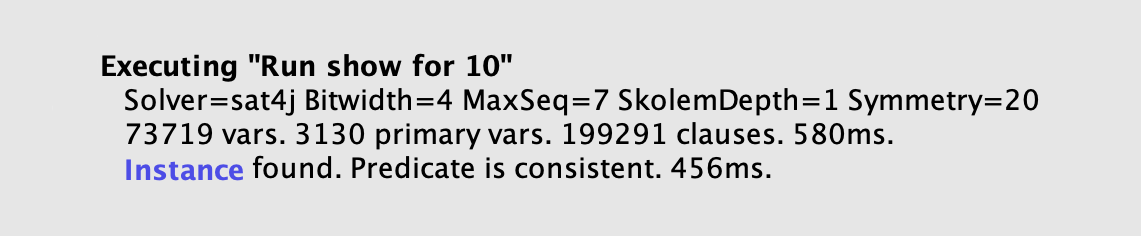
\includegraphics{assets/rasd/alloy/execution_result.png}
\caption{Execution result}
\end{figure}

\hypertarget{c.-generated-worlds}{%
\subsubsection{C. Generated worlds}\label{c.-generated-worlds}}

\hypertarget{c.1.-world-1}{%
\paragraph{C.1. World 1}\label{c.1.-world-1}}

\begin{figure}
\centering
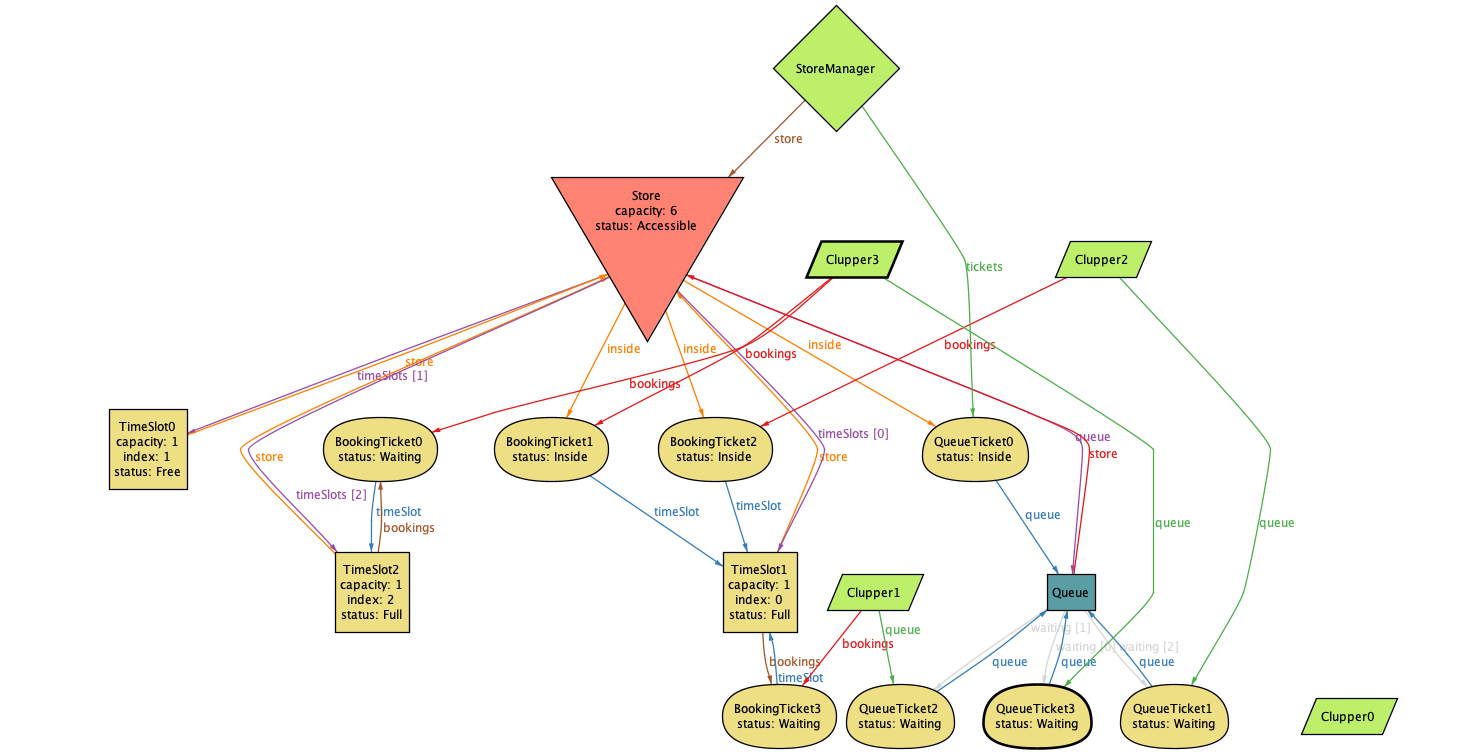
\includegraphics{assets/rasd/alloy/world_1.png}
\caption{World 1}
\end{figure}

\hypertarget{c.2.-world-2}{%
\paragraph{C.2. World 2}\label{c.2.-world-2}}

\begin{figure}
\centering
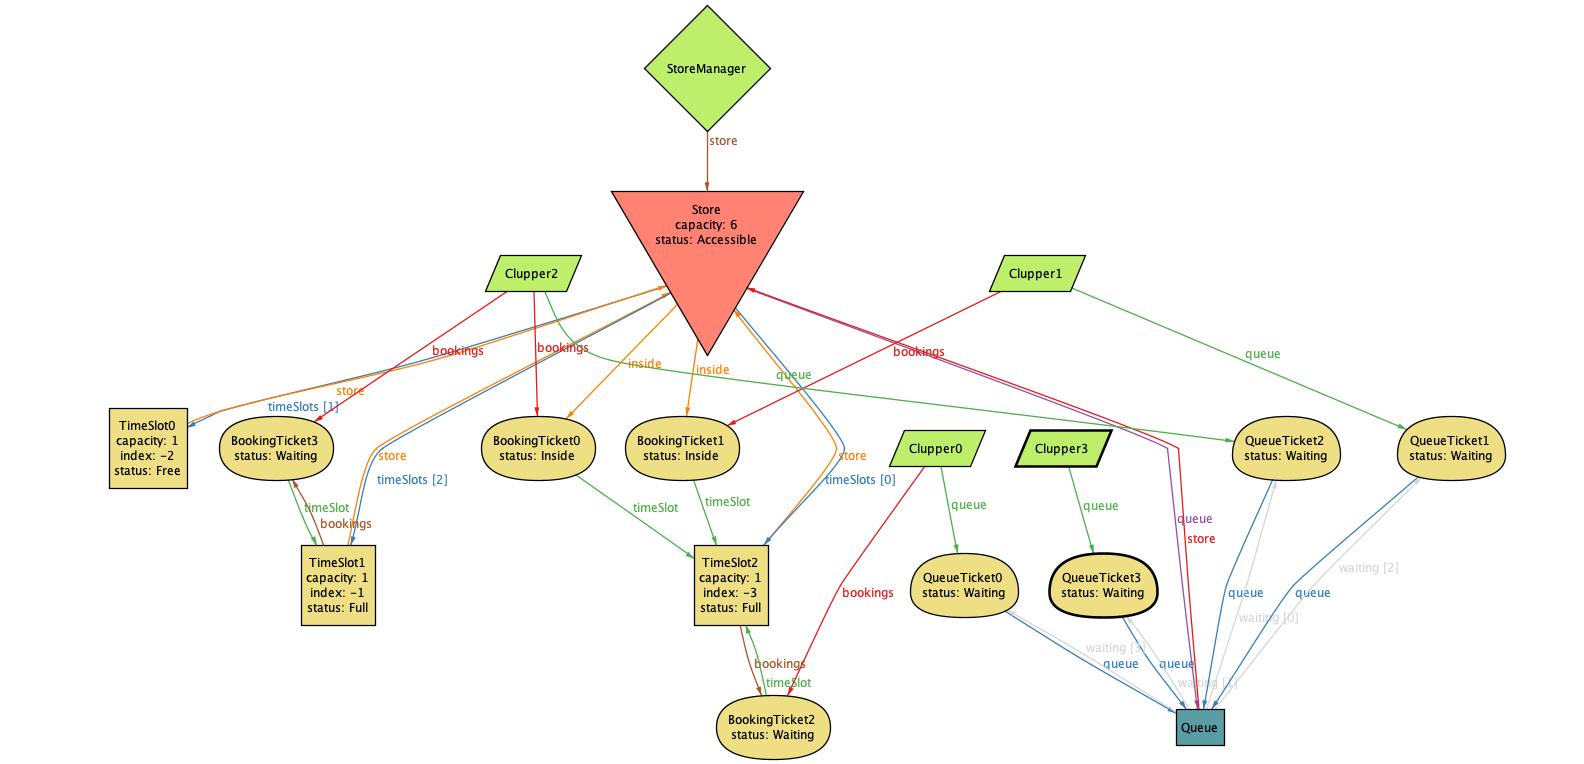
\includegraphics{assets/rasd/alloy/world_2.png}
\caption{World 2}
\end{figure}

\hypertarget{effort-spent}{%
\subsection{5. Effort spent}\label{effort-spent}}

\hypertarget{pair-programming}{%
\subsubsection{Pair programming}\label{pair-programming}}

\begin{longtable}[]{@{}lr@{}}
\toprule
Topic & Hours \\ \addlinespace
\midrule
\endhead
Discussion on the first part & 1.5h \\ \addlinespace
First and second part & 2.5h \\ \addlinespace
Second and third part & 2.5h \\ \addlinespace
Domain assumption, functional requirements and mapping &
2.0h \\ \addlinespace
Structure adaptation, edit on previous parts, more on third part &
2.5h \\ \addlinespace
Scenarios and use cases & 3.0h \\ \addlinespace
Overall RASD revision & 3.5h \\ \addlinespace
Scenarios and use cases revision & 1.5h \\ \addlinespace
Alloy & 2.0h \\ \addlinespace
\bottomrule
\end{longtable}

\hypertarget{ferrara-alessandro}{%
\subsubsection{Ferrara Alessandro}\label{ferrara-alessandro}}

\begin{longtable}[]{@{}lr@{}}
\toprule
Topic & Hours \\ \addlinespace
\midrule
\endhead
Sequence Diagrams & 3.0h \\ \addlinespace
Use Cases & 1.0h \\ \addlinespace
Alloy & 2.0h \\ \addlinespace
\bottomrule
\end{longtable}

\hypertarget{fratus-lorenzo}{%
\subsubsection{Fratus Lorenzo}\label{fratus-lorenzo}}

\begin{longtable}[]{@{}lr@{}}
\toprule
Topic & Hours \\ \addlinespace
\midrule
\endhead
Mockup UI & 4.0h \\ \addlinespace
State diagrams & 2.0h \\ \addlinespace
Scenarios & 1.5h \\ \addlinespace
Alloy & 6.0h \\ \addlinespace
RASD revision & 1.0h \\ \addlinespace
\bottomrule
\end{longtable}

\hypertarget{references}{%
\subsection{6. References}\label{references}}

\begin{itemize}
\tightlist
\item
  Software Engineering II course slides
\item
  \href{https://www.gazzettaufficiale.it/atto/vediPermalink?atto.dataPubblicazioneGazzetta=2020-11-09\&atto.codiceRedazionale=20G00170\&tipoSerie=serie_generale\&tipoVigenza=originario\&tipoProvvedimento=*}{Decreto
  Ministeriale}
\end{itemize}

\end{document}
